% ============================================================================
% BÀI BÁO KHOA HỌC — TEMPLATE IEEEtran CHUẨN (JOURNAL / A4) CHO OVERLEAF
% Hỗ trợ 100% tiếng Việt có dấu sắc nét (pdfLaTeX + T5 + Times TeX Gyre Termes)
% Hướng dẫn biên dịch trên Overleaf:
%   1. Tải gói nén Vi_ESG_Bert_Overleaf_Paper.zip lên Overleaf (Upload Project)
%      HOẶC dán đè nội dung main.tex này vào dự án đã có thư mục figures/.
%   2. Menu -> Compiler: chọn "pdfLaTeX" (mặc định của Overleaf).
%   3. Nhấn Recompile -> Xuất PDF chuẩn IEEE Transactions 2 cột tiếng Việt.
% ============================================================================
\documentclass[journal,a4paper]{IEEEtran}

% --- Gói hỗ trợ tiếng Việt có dấu chuẩn IEEE (Times New Roman vector T5) ---
\usepackage[utf8]{inputenc}
\usepackage[T5]{fontenc}
\usepackage[vietnamese]{babel}
\usepackage{tgtermes}

% --- Toán học, bảng biểu, trích dẫn IEEE, thuật toán, đồ họa ---
\usepackage{amsmath,amssymb,amsfonts}
\usepackage{cite}
\usepackage{graphicx}
\usepackage{booktabs}
\usepackage{array}
\usepackage{tabularx}
\usepackage{adjustbox}
\usepackage{xcolor}
\usepackage{algorithm}
\usepackage{algpseudocode}
\usepackage{enumitem}
\usepackage{dblfloatfix}
\usepackage{balance}

% --- Liên kết chéo tương thích Unicode tiếng Việt ---
\usepackage[
  unicode,
  pdfencoding=auto,
  colorlinks=true,
  linkcolor=blue!55!black,
  citecolor=teal!65!black,
  urlcolor=blue!60!black
]{hyperref}

% --- Tăng giới hạn hàng đợi float và tối ưu phân bố hình/bảng 2 cột ---
\extrafloats{50}
\setcounter{topnumber}{3}
\setcounter{dbltopnumber}{2}
\renewcommand{\topfraction}{0.90}
\renewcommand{\dbltopfraction}{0.92}
\renewcommand{\textfraction}{0.07}
\renewcommand{\floatpagefraction}{0.75}
\renewcommand{\dblfloatpagefraction}{0.75}

% --- Việt hóa đầy đủ các nhãn chuẩn của IEEEtran và thuật toán ---
\floatname{algorithm}{Thuật toán}
\renewcommand{\algorithmicrequire}{\textbf{Đầu vào:}}
\renewcommand{\algorithmicensure}{\textbf{Đầu ra:}}
\AtBeginDocument{%
  \renewcommand{\abstractname}{Tóm tắt}%
  \renewcommand{\IEEEkeywordsname}{Từ khóa}%
  \renewcommand{\figurename}{Hình}%
  \renewcommand{\tablename}{BẢNG}%
  \renewcommand{\refname}{Tài liệu tham khảo}%
}

% --- Đường dẫn ảnh vector PDF ---
\graphicspath{{figures/}}

% --- Macro định dạng nhanh ---
\newcommand{\best}[1]{\textbf{#1}}
\newcommand{\code}[1]{\texttt{\small #1}}

% ============================================================================
\begin{document}

% --- TIÊU ĐỀ, TÁC GIẢ VÀ TIÊU ĐỀ ĐẦU TRANG CHUẨN IEEE TRANSACTIONS ---
\title{Phân loại văn bản ESG tiếng Việt bằng học bán giám sát lặp\\
kết hợp đồng thuận đa mô hình Transformer}

\author{Lưu~Tuấn~Trình%
\thanks{Lưu Tuấn Trình thực hiện nghiên cứu này trong khuôn khổ đồ án môn Xử lý ngôn ngữ tự nhiên (hệ thống Vi-ESG-Bert). Thực nghiệm được tiến hành trên GPU NVIDIA GeForce RTX 5070 (12~GB VRAM), PyTorch 2.11 và Transformers 5.24.}}

\markboth{BÁO CÁO NGHIÊN CỨU KHOA HỌC --- XỬ LÝ NGÔN NGỮ TỰ NHIÊN (VI-ESG-BERT)}%
{Lưu Tuấn Trình: Phân loại văn bản ESG tiếng Việt bằng học bán giám sát lặp kết hợp đồng thuận đa mô hình}

\maketitle

% --- TÓM TẮT VÀ TỪ KHÓA CHUẨN IEEEtran ---
\begin{abstract}
Phân loại tự động văn bản doanh nghiệp tiếng Việt theo bốn hạng mục ESG (\textit{Không liên quan, Môi trường, Xã hội, Quản trị}) phục vụ công tác định lượng phát triển bền vững, nhưng thường gặp hai trở ngại chính: (i) chi phí gán nhãn chuyên gia cao khiến dữ liệu có nhãn bị giới hạn trong khi kho văn bản không nhãn lớn hơn nhiều, và (ii) sự mất cân bằng lớp kết hợp dịch chuyển xác suất tiên nghiệm (\textit{Prior Probability Shift}) giữa tập huấn luyện và tập kiểm thử. Nghiên cứu này trình bày một quy trình thực nghiệm không rò rỉ dữ liệu (\textit{Zero Data Leakage}), áp dụng phương pháp học bán giám sát lặp kết hợp đồng thuận đa mô hình (\textit{Iterative Ensemble Pseudo-Labeling}) qua ba vòng trên bảy kiến trúc Transformer (bốn mô hình tiếng Việt và ba mô hình đa ngôn ngữ hoặc tiếng Anh), kèm thực nghiệm đối chứng có giám sát (\textit{Ablation Study}). Kết quả kiểm toán 84.856 câu gốc thu được 27.365 mẫu huấn luyện sạch, 3.000 mẫu kiểm thử khóa kín và 54.487 câu không nhãn sạch với 0 mẫu trùng lặp chéo giữa các tập. Sau khi khắc phục lỗi nạp trọng số \code{float16} trên \code{Transformers 5.24.0}, hai vòng bỏ phiếu đồng thuận đã chọn lọc 32.903/54.487 câu không nhãn (60,4\%, trong đó vòng~2 có 97,52\% mẫu đạt đồng thuận 7/7 mô hình), hình thành tập huấn luyện cuối 39.248 mẫu và giảm tỷ số mất cân bằng $IR$ từ $2{,}29$ xuống $1{,}61$ rồi $1{,}35$, tiệm cận phân phối tập kiểm thử ($1{,}42$). Trên tập kiểm thử khóa kín (3.000 mẫu), cả bảy mô hình ở vòng~3 đều cải thiện so với các mốc đối chứng có giám sát trên 100\% tập huấn luyện gốc (\code{PhoBERT-base} tăng $+1{,}67\%$, \code{Vi-ELECTRA} tăng $+1{,}50\%$, \code{ViSoBERT} tăng $+4{,}56\%$ Macro-F1); trong nhóm mô hình đơn lẻ, \code{DistilBERT-m} đạt kết quả cao nhất với 89,70\% Accuracy và 89,03\% Macro-F1 tại độ trễ 0,324~ms/câu (3.085~mẫu/giây). Mô hình kết hợp trung bình xác suất đồng đều 7 mô hình (\code{Equal Soft 7M}) đạt 90,77\% Accuracy, 90,09\% Macro-F1 và 90,67\% Weighted-F1, cao hơn có ý nghĩa thống kê so với mô hình đơn lẻ tốt nhất ($+1{,}06\%$ Macro-F1, kiểm định McNemar $\chi^2 = 5{,}79, p = 0{,}0161 < 0{,}05$) và mốc đối chứng mạnh nhất ($+3{,}63\%$ Macro-F1, $\chi^2 = 32{,}95, p < 10^{-6}$), đồng thời giảm sai số hiệu chuẩn xác suất (ECE) xuống 0,0226 so với mức 0,0825--0,1117 ở các mô hình đơn lẻ. Phân tích 277 mẫu dự đoán sai (9,23\%) cho thấy 82,31\% lỗi tập trung tại bốn cặp lớp biên, liên quan đến dấu hiệu nhiễu nhãn trong tập kiểm thử gốc, tính giao thoa đa nhãn giữa \textit{Xã hội} và \textit{Quản trị}, cùng sự trùng lặp thuật ngữ kế toán--tài chính.
\end{abstract}

\begin{IEEEkeywords}
Phân loại văn bản ESG tiếng Việt, học bán giám sát, gán nhãn giả lặp (Iterative Pseudo-Labeling), học kết hợp (Ensemble Learning), hiệu chuẩn xác suất (ECE), kiểm định McNemar, dịch chuyển phân phối lớp.
\end{IEEEkeywords}

\IEEEpeerreviewmaketitle

% ============================================================================
\section{Giới thiệu}
\label{sec:intro}

\IEEEPARstart{T}{rong} lĩnh vực tài chính bền vững và công bố thông tin phi tài chính, nhu cầu phân loại tự động các câu văn trong báo cáo thường niên, báo cáo phát triển bền vững và tin tức doanh nghiệp tiếng Việt thành bốn hạng mục ESG --- gồm \textit{Không liên quan} (\code{Irrelevant}, lớp~0), \textit{Môi trường} (\code{Environment}, lớp~1), \textit{Xã hội} (\code{Social}, lớp~2) và \textit{Quản trị} (\code{Governance}, lớp~3) --- có vai trò quan trọng trong đánh giá rủi ro và chấm điểm mức độ bền vững của doanh nghiệp~\cite{huang2023finbert}.

Tuy vậy, việc xây dựng hệ thống phân loại văn bản ESG tiếng Việt có độ tin cậy cao gặp ba thách thức phương pháp luận chính:
\begin{enumerate}[leftmargin=*, itemsep=2pt, topsep=2pt]
  \item \textbf{Hạn chế về dữ liệu có nhãn so với dữ liệu không nhãn:} Việc gán nhãn ESG đòi hỏi kiến thức chuyên ngành về môi trường, lao động và quản trị doanh nghiệp, do đó số lượng câu có nhãn thường nhỏ hơn đáng kể so với kho văn bản không nhãn sẵn có.
  \item \textbf{Mất cân bằng lớp và dịch chuyển phân phối:} Trong tập dữ liệu nghiên cứu, tập huấn luyện gốc có tỷ số mất cân bằng $IR = 2{,}29$ (lớp \textit{Social} chiếm 36,64\% trong khi lớp \textit{Environment} chiếm 16,02\%), còn tập kiểm thử có phân phối cân bằng hơn ($IR = 1{,}42$, trong đó tỷ trọng \textit{Environment} tăng thêm $+11{,}31$ điểm phần trăm và \textit{Social} giảm $-8{,}31$ điểm phần trăm). Bên cạnh dịch chuyển xác suất tiên nghiệm (\textit{Prior Probability Shift}), độ dài câu trung bình của tập kiểm thử và tập không nhãn cũng lớn hơn tập huấn luyện (\textit{Covariate Length Shift}).
  \item \textbf{Nguy cơ rò rỉ dữ liệu và hiện tượng quá tự tin:} Nếu quy trình bán giám sát không tách tập kiểm định (\textit{validation}) độc lập, sử dụng tập kiểm thử để chọn trọng số, hoặc tạo nhãn giả chỉ từ một mô hình đơn lẻ, hệ thống dễ gặp thiên lệch xác nhận (\textit{confirmation bias}) và sai lệch hiệu chuẩn xác suất (\textit{over-confidence})~\cite{guo2017calibration}.
\end{enumerate}

Để giải quyết các vấn đề nêu trên, nghiên cứu này chuẩn hóa quy trình \textbf{Vi-ESG-Bert} với năm nội dung đóng góp chính:
\begin{itemize}[leftmargin=*, itemsep=2pt, topsep=2pt]
  \item \textbf{Kiểm toán không rò rỉ dữ liệu:} Thực hiện kiểm tra trùng lặp nội bộ, mâu thuẫn nhãn và trùng lặp chéo trên toàn bộ 84.856 câu; khóa kín tập kiểm thử 3.000 câu và tách phân tầng 90/10 độc lập từ tập huấn luyện sạch để chọn checkpoint theo chỉ số \code{Macro-F1}.
  \item \textbf{Tiền xử lý đồng nhất theo kiến trúc:} Quy chuẩn bảng mã Unicode NFC cho toàn bộ văn bản, chỉ áp dụng tách từ tiếng Việt bằng \code{pyvi} cho mô hình tiền huấn luyện ở mức từ (\code{PhoBERT-base}) và giữ nguyên văn bản tự nhiên cho sáu mô hình subword/SentencePiece ở mọi giai đoạn huấn luyện, gán nhãn giả và suy luận.
  \item \textbf{Học bán giám sát lặp kết hợp đồng thuận đa mô hình và cân bằng lớp:} Khai thác 54.487 câu không nhãn qua hai vòng bỏ phiếu kết hợp giữa bảy kiến trúc Transformer (đồng thuận cứng, trung bình xác suất có trọng số, biên độ xác suất và cổng chất lượng), đồng thời chọn lọc nhãn giả theo độ tin cậy giảm dần để đưa tỷ số mất cân bằng $IR$ từ $2{,}29$ về $1{,}35$.
  \item \textbf{Nghiên cứu đối chứng và kiểm định thống kê:} Bổ sung mốc huấn luyện có giám sát trên 100\% tập huấn luyện gốc không dùng nhãn giả nhằm định lượng phần cải thiện thực chất của nhãn giả và kiểm chứng ý nghĩa thống kê bằng kiểm định McNemar hai phía.
  \item \textbf{Đánh giá định hướng triển khai:} Kết hợp đánh giá hiệu chuẩn xác suất (Reliability Diagram và ECE), phân tích đánh đổi hiệu năng--độ trễ trên đường biên Pareto và phân tích lỗi định lượng lẫn định tính.
\end{itemize}

% ============================================================================
\section{Nghiên cứu liên quan}
\label{sec:related}

\textbf{Mô hình ngôn ngữ tiền huấn luyện cho tiếng Việt và đa ngôn ngữ.} Các mô hình dựa trên kiến trúc Transformer là nền tảng phổ biến cho bài toán phân loại văn bản. Nhóm mô hình đa ngôn ngữ như \code{mBERT}~\cite{devlin2019bert}, \code{DistilBERT-m}~\cite{sanh2019distilbert} và mô hình tiếng Anh \code{RoBERTa}~\cite{liu2019roberta} có ưu thế khi xử lý văn bản tài chính chứa thuật ngữ tiếng Anh hoặc tên tổ chức quốc tế. Đối với tiếng Việt, \code{PhoBERT}~\cite{nguyen2020phobert} được tiền huấn luyện ở mức từ trên ngữ liệu 20~GB; \code{Vi-ELECTRA} kế thừa cơ chế phát hiện token thay thế (\textit{Replaced Token Detection}) của kiến trúc ELECTRA~\cite{clark2020electra}; \code{ViSoBERT}~\cite{nguyen2023visobert} tập trung vào văn bản mạng xã hội và tin tức tiếng Việt hiện đại; còn \code{ViDeBERTa}~\cite{tran2023videberta} sử dụng cơ chế chú ý tách biệt (\textit{Disentangled Attention}) của DeBERTa-v2. Sự khác nhau về bộ tách từ và mục tiêu tiền huấn luyện giữa bảy kiến trúc này tạo ra tính đa dạng (\textit{ensemble diversity}) có lợi cho các phương pháp học kết hợp~\cite{dietterich2000ensemble}.

\textbf{Học bán giám sát bằng nhãn giả và học kết hợp.} Lee~\cite{lee2013pseudo} giới thiệu kỹ thuật tự gán nhãn giả cho dữ liệu không nhãn và chỉ ra mối liên hệ với nguyên lý tối thiểu hóa entropy~\cite{grandvalet2004semi}. Trong thực tế, việc sinh nhãn giả từ một mô hình duy nhất dễ bị ảnh hưởng bởi các dự đoán sai nhưng có xác suất cao do mạng nơ-ron sâu thường bị lệch hiệu chuẩn~\cite{guo2017calibration}. Do đó, kết hợp đồng thuận từ nhiều kiến trúc khác nhau giúp giảm nhiễu nhãn giả và cải thiện độ hiệu chuẩn xác suất. Nghiên cứu này mở rộng cách tiếp cận trên bằng cơ chế chọn lọc nhãn giả cân bằng theo lớp nhằm đồng thời khắc phục mất cân bằng dữ liệu và dịch chuyển xác suất tiên nghiệm.

% ============================================================================
\section{Phương pháp đề xuất}
\label{sec:method}

\subsection{Thiết kế giao thức chống rò rỉ dữ liệu và tiền xử lý}
\label{sec:method_leakage}

Gọi $\mathcal{D}_{\text{train}}^{\text{raw}}$, $\mathcal{D}_{\text{test}}^{\text{raw}}$ và $\mathcal{D}_{U}^{\text{raw}}$ lần lượt là ba tập dữ liệu huấn luyện, kiểm thử và không nhãn ban đầu. Mọi câu $x$ được chuyển về chuẩn mã hóa Unicode NFC và chuẩn hóa khoảng trắng. Hệ thống tạo khóa đối chiếu $k(x)$ (chữ thường, loại bỏ dấu câu thừa) để kiểm toán và lọc theo bốn bước: (1) loại bỏ câu rỗng hoặc có dưới 5 từ; (2) loại bỏ các mẫu trùng khóa nhưng có nhãn mâu thuẫn; (3) khử trùng lặp nội bộ trong từng tập; và (4) loại bỏ mọi mẫu trong $\mathcal{D}_{\text{train}}$ hoặc $\mathcal{D}_{U}$ có khóa trùng với $\mathcal{D}_{\text{test}}$, cũng như mẫu trong $\mathcal{D}_{U}$ trùng với $\mathcal{D}_{\text{train}}$.

Từ tập huấn luyện sạch $\mathcal{D}_{\text{train}}$, hệ thống chia phân tầng theo tỷ lệ 90/10 (\code{seed=42}) thành tập huấn luyện gốc $\mathcal{D}_{L}$ (24.628 mẫu) và tập kiểm định cố định $\mathcal{D}_{\text{val}}$ (2.737 mẫu). Tập kiểm thử $\mathcal{D}_{\text{test}}$ (3.000 mẫu) được giữ độc lập hoàn toàn, chỉ sử dụng để đo lường kết quả đánh giá sau khi kết thúc mỗi vòng huấn luyện.

Về tiền xử lý theo kiến trúc, gọi $\phi_m(x)$ là hàm biến đổi đầu vào cho mô hình thứ $m \in \{1,\dots,M\}$ ($M = 7$). Ta định nghĩa $\phi_m(x) = \text{ViTokenizer}(\text{NFC}(x))$ nếu $m$ là \code{PhoBERT-base}, và $\phi_m(x) = \text{NFC}(x)$ cho sáu mô hình còn lại. Quy tắc này được đóng gói thống nhất trong module \code{src/preprocessing.py} để tránh sai lệch biểu diễn giữa huấn luyện và suy luận.

\subsection{Mô hình hóa Iterative Ensemble Pseudo-Labeling}
\label{sec:method_algo}

Quy trình gồm ba vòng huấn luyện ($r \in \{1, 2, 3\}$) xen kẽ hai vòng sinh nhãn giả đồng thuận ($t \in \{1, 2\}$):

\textbf{Khởi tạo đa dạng ở vòng~1 ($r=1$):} Từ $\mathcal{D}_{L}$, hệ thống lấy mẫu ngẫu nhiên bảy tập con $\mathcal{D}_{L}^{(m)}$, mỗi tập 10.000 mẫu cho từng mô hình $m=1,\dots,7$. Mỗi mô hình $f_m^{(1)}$ được tinh chỉnh độc lập và lưu checkpoint có $\text{Macro-F1}$ cao nhất trên $\mathcal{D}_{\text{val}}$. Song song đó, ba mô hình tiếng Việt (\code{PhoBERT-base}, \code{Vi-ELECTRA} và \code{ViSoBERT}) được huấn luyện trên 100\% $\mathcal{D}_{L}$ (không bổ sung nhãn giả) làm nhóm đối chứng có giám sát (\textit{Ablation Baseline}).

\textbf{Tính trọng số có cổng chất lượng (\textit{Quality Gate}):} Tại vòng gán nhãn giả $t \in \{1,2\}$, gọi $s_m^{(t)} = \text{Macro-F1}(f_m^{(t)}, \mathcal{D}_{\text{val}})$ là điểm kiểm định của mô hình $m$. Để ngăn một mô hình không hội tụ ảnh hưởng đến kết quả tổng hợp, trọng số được xác định qua cổng chất lượng với ngưỡng $\gamma = 0{,}50$:
\begin{equation}
  w_m^{(t)} = \frac{\mathbb{I}\!\left(s_m^{(t)} \ge \gamma\right) \cdot s_m^{(t)}}{\sum_{j=1}^{M} \mathbb{I}\!\left(s_j^{(t)} \ge \gamma\right) \cdot s_j^{(t)}}
  \label{eq:weights}
\end{equation}

\textbf{Bỏ phiếu đồng thuận đa tiêu chuẩn:} Với mỗi câu không nhãn $u \in \mathcal{U}^{(t)}$, mô hình $m$ cho phân phối xác suất hậu nghiệm $\mathbf{p}_m(u) = (p_{m,0}(u), \dots, p_{m,3}(u)) \in \Delta^3$ và nhãn dự đoán cứng $\hat{y}_m(u) = \arg\max_c p_{m,c}(u)$. Phân phối xác suất tổng hợp có trọng số là:
\begin{equation}
  \bar{\mathbf{p}}^{(t)}(u) = \sum_{m=1}^{M} w_m^{(t)}\,\mathbf{p}_m(u)
  \label{eq:softprob}
\end{equation}
Đặt $\hat{y}(u) = \arg\max_c \bar{p}_c^{(t)}(u)$, độ tin cậy lớn nhất $c_{\max}(u) = \max_c \bar{p}_c^{(t)}(u)$, xác suất lớn thứ hai $c_{(2)}(u)$, và số phiếu đồng thuận cứng $v(u) = \sum_{m} \mathbb{I}(\hat{y}_m(u) = \hat{y}(u))$. Câu $u$ được đưa vào tập nhãn giả $\mathcal{P}^{(t)}$ khi thỏa đồng thời ba điều kiện:
\begin{equation}
  c_{\max}(u) \ge \tau_t, \quad c_{\max}(u) - c_{(2)}(u) \ge \delta_t, \quad v(u) \ge V_{\min}
  \label{eq:filter}
\end{equation}
Cụ thể, vòng~1 áp dụng $(\tau_1 = 0{,}94, \delta_1 = 0{,}50, V_{\min} = 5/7)$, còn vòng~2 thực hiện trên phần dư $\mathcal{U}^{(2)} = \mathcal{U}^{(1)} \setminus \mathcal{P}^{(1)}$ với $(\tau_2 = 0{,}91, \delta_2 = 0{,}45, V_{\min} = 5/7)$.

\textbf{Gộp cân bằng lớp có chọn lọc:} Gọi $N_c^{(t)}$ là số mẫu hiện có của lớp $c \in \{0,1,2,3\}$ trước khi gộp và $T_t$ là chỉ tiêu số mẫu mỗi lớp ($T_1 = 9.500$, $T_2 = 10.500$). Trong mỗi lớp $c$, hệ thống sắp xếp các mẫu ứng viên thuộc $\mathcal{P}^{(t)}_c$ theo chiều giảm dần của $c_{\max}(u)$ và chọn tối đa $\Delta_c^{(t)} = \max(0, T_t - N_c^{(t)})$ mẫu có độ tin cậy cao nhất để ghép vào tập huấn luyện mới $\mathcal{D}_{\text{comb}}^{(t)}$. Ở các vòng huấn luyện sau ($r=2,3$), toàn bộ bảy mô hình đều được khởi tạo lại từ trọng số tiền huấn luyện ban đầu nhằm hạn chế quá khớp tích lũy. Quy trình chi tiết được mô tả trong Thuật toán~\ref{alg:iepl}.

\begin{algorithm}[!t]
\caption{Học bán giám sát lặp kết hợp đồng thuận đa mô hình cân bằng lớp}
\label{alg:iepl}
\begin{algorithmic}[1]
\Require $\mathcal{D}_{L}$ (24.628), $\mathcal{D}_{\text{val}}$ (2.737), $\mathcal{U}^{(1)}$ (54.487), bảy kiến trúc $\{f_m\}_{m=1}^7$, chỉ tiêu $(T_1, T_2)$
\Ensure Bảy mô hình vòng~3 $\{f_m^{(3)}\}$ và mô hình kết hợp $F^*$
\State Trích bảy tập con $\mathcal{D}_L^{(m)}$ (10.000 mẫu); huấn luyện $\{f_m^{(1)}\}$ và chọn checkpoint theo $\text{Macro-F1}(\mathcal{D}_{\text{val}})$
\State $\mathcal{D}_{\text{curr}} \leftarrow \mathcal{D}_L$
\For{$t \in \{1, 2\}$}
  \State Tính trọng số $w_m^{(t)}$ qua cổng chất lượng ($\gamma = 0{,}50$) theo (\ref{eq:weights})
  \State Suy luận $\mathbf{p}_m(u)$ trên $\mathcal{U}^{(t)}$ và tổng hợp $\bar{\mathbf{p}}^{(t)}(u)$ theo (\ref{eq:softprob})
  \State Lọc $\mathcal{P}^{(t)}$ theo (\ref{eq:filter}); cập nhật phần dư $\mathcal{U}^{(t+1)} \leftarrow \mathcal{U}^{(t)} \setminus \mathcal{P}^{(t)}$
  \For{$c \in \{0, 1, 2, 3\}$}
    \State Sắp xếp $\mathcal{P}_c^{(t)}$ giảm dần theo $c_{\max}(u)$
    \State Chọn tối đa $\max(0, T_t - |\mathcal{D}_{\text{curr}, c}|)$ mẫu ghép vào $\mathcal{D}_{\text{curr}}$
  \EndFor
  \State Khởi tạo lại từ trọng số tiền huấn luyện và huấn luyện $\{f_m^{(t+1)}\}$ trên $\mathcal{D}_{\text{curr}}$
\EndFor
\State Kết hợp $\{f_m^{(3)}\}$ thành mô hình $F^*$; đánh giá cuối cùng trên $\mathcal{D}_{\text{test}}$
\end{algorithmic}
\end{algorithm}

\subsection{Chỉ số đánh giá, hiệu chuẩn xác suất và kiểm định thống kê}
\label{sec:method_metrics}

Ngoài các chỉ số phân loại chuẩn gồm \code{Accuracy}, \code{Macro-F1} (chỉ số ưu tiên do dữ liệu mất cân bằng) và \code{Weighted-F1}, nghiên cứu sử dụng hai công cụ đánh giá bổ sung:

\textbf{Sai số hiệu chuẩn kỳ vọng (\textit{Expected Calibration Error} --- ECE):} Chia khoảng xác suất $[0,1]$ thành $B=10$ khoảng đều $I_b$:
\begin{equation}
  \text{ECE} = \sum_{b=1}^{B} \frac{|I_b|}{N} \left|\,\text{acc}(I_b) - \text{conf}(I_b)\,\right|
  \label{eq:ece}
\end{equation}
Giá trị ECE càng nhỏ chứng tỏ xác suất dự đoán của mô hình càng phản ánh sát xác suất đoán đúng thực tế~\cite{guo2017calibration}.

\textbf{Kiểm định McNemar với hiệu chỉnh liên tục Edwards:} Khi so sánh hai mô hình $A$ và $B$ trên cùng $N = 3.000$ mẫu kiểm thử, gọi $n_{10}$ là số mẫu chỉ $A$ đoán đúng ($B$ đoán sai) và $n_{01}$ là số mẫu chỉ $B$ đoán đúng ($A$ đoán sai):
\begin{equation}
  \chi^2 = \frac{(|n_{10} - n_{01}| - 1)^2}{n_{10} + n_{01}}
  \label{eq:mcnemar}
\end{equation}
Sự khác biệt được xem là có ý nghĩa thống kê ở mức $\alpha = 0{,}05$ khi $p < 0{,}05$~\cite{mcnemar1947note}.

% ============================================================================
\section{Thiết lập thực nghiệm và kiểm toán dữ liệu}
\label{sec:setup}

\subsection{Hạ tầng tính toán và cấu hình bảy mô hình}

Thực nghiệm được triển khai trên máy trạm Windows~11 (20 luồng CPU), GPU NVIDIA GeForce RTX 5070 (11,94~GB VRAM, kiến trúc Blackwell Compute Capability 12.0), Python~3.14.7, PyTorch~2.11.0+cu128 và Transformers~5.24.0. Cấu hình mặc định sử dụng độ chính xác hỗn hợp \code{bf16=True}, kích thước lô \code{batch\_size=16} kết hợp \code{grad\_accum=2} (kích thước lô hiệu dụng bằng 32), \code{max\_length=256}, \code{warmup=10\%}, tốc độ học \code{lr=2e-5} (riêng \code{ViDeBERTa-base} dùng \code{lr=1.5e-5} và \code{activation\_checkpointing=True}), tối đa 8~epoch với dừng sớm \code{EarlyStopping(patience=2)} theo \code{Val Macro-F1} và hạt giống ngẫu nhiên \code{seed=42}. Thông số của bảy mô hình được tổng hợp tại Bảng~\ref{tab:models}.

\begin{table*}[!t]
\centering
\caption{Danh mục bảy kiến trúc Transformer trong hệ thống Vi-ESG-Bert và vai trò bổ trợ trong tập thể.}
\label{tab:models}
\footnotesize
\renewcommand{\arraystretch}{1.15}
\setlength{\tabcolsep}{4pt}
\begin{adjustbox}{max width=\textwidth}
\begin{tabular}{@{}clllccl@{}}
\toprule
\textbf{STT} & \textbf{Tên mô hình} & \textbf{Checkpoint HuggingFace} & \textbf{Họ kiến trúc} & \textbf{Tham số} & \textbf{\code{pyvi}} & \textbf{Đặc trưng bổ trợ trong tập thể} \\
\midrule
1 & PhoBERT-base & \code{vinai/phobert-base} & RoBERTa (VN) & 135,0M & Có & Xử lý tốt ngữ pháp và từ ghép tiếng Việt chuẩn \\
2 & Vi-ELECTRA & \code{NlpHUST/electra-base-vn} & ELECTRA (VN) & 133,7M & Không & Biểu diễn ngữ nghĩa hiệu quả qua cơ chế RTD \\
3 & ViSoBERT & \code{uitnlp/visobert} & XLM-R (VN) & 97,6M & Không & Gọn nhẹ, thích hợp với tin tức và văn bản truyền thông \\
4 & ViDeBERTa-base & \code{Fsoft-AIC/videberta-base} & DeBERTa-v2 (VN) & 184,3M & Không & Cơ chế chú ý tách biệt, độ hiệu chuẩn xác suất tốt \\
5 & mBERT-cased & \code{google-bert/bert-base-multilingual-cased} & BERT (Multi) & 177,9M & Không & Biểu diễn đa ngôn ngữ và thuật ngữ ESG quốc tế \\
6 & DistilBERT-m & \code{distilbert/distilbert-base-multilingual-cased} & DistilBERT (6 lớp) & 135,3M & Không & Tốc độ suy luận cao, mốc tham chiếu đường biên Pareto \\
7 & RoBERTa-base & \code{FacebookAI/roberta-base} & RoBERTa (EN) & 124,6M & Không & Tăng đa dạng kiến trúc và nhận diện từ tiếng Anh xen kẽ \\
\bottomrule
\end{tabular}
\end{adjustbox}
\end{table*}

\subsection{Kiểm toán dữ liệu và phân tích khám phá phân phối}

\begin{table}[!t]
\centering
\caption{Kết quả kiểm toán làm sạch và xác minh không rò rỉ dữ liệu trên 84.856 mẫu gốc.}
\label{tab:audit}
\footnotesize
\renewcommand{\arraystretch}{1.15}
\setlength{\tabcolsep}{3.5pt}
\begin{adjustbox}{max width=\columnwidth}
\begin{tabular}{@{}lccccc@{}}
\toprule
\textbf{Tập dữ liệu} & \textbf{Gốc} & \textbf{Rỗng/Ngắn} & \textbf{Trùng} & \textbf{Rò rỉ} & \textbf{Sạch} \\
\midrule
Train (\code{train.csv}) & 27.366 & 0 & 1 & \textbf{0} & \textbf{27.365} \\
Test (\code{test.csv}) & 3.000 & 0 & 0 & \textbf{0} & \textbf{3.000} \\
Unlabeled (\code{overall}) & 54.490 & 0 & 3 & \textbf{0} & \textbf{54.487} \\
\midrule
\textbf{Tổng cộng} & \textbf{84.856} & \textbf{0} & \textbf{4} & \textbf{0} & \textbf{84.852} \\
\bottomrule
\end{tabular}
\end{adjustbox}
\end{table}

\begin{table}[!t]
\centering
\caption{Phân bố bốn lớp ESG và mức độ dịch chuyển xác suất tiên nghiệm giữa tập huấn luyện và tập kiểm thử.}
\label{tab:dist}
\footnotesize
\renewcommand{\arraystretch}{1.15}
\setlength{\tabcolsep}{3.5pt}
\begin{adjustbox}{max width=\columnwidth}
\begin{tabular}{@{}lcccc@{}}
\toprule
\textbf{Lớp ESG} & \textbf{Train Pool} & \textbf{Val (10\%)} & \textbf{Test} & \textbf{Lệch (T$-$Tr)} \\
\midrule
0 -- Irrelevant & 5.312 (21,57\%) & 590 (21,56\%) & 600 (20,00\%) & $-1{,}57\%$ \\
1 -- Environment & 3.945 (16,02\%) & 439 (16,04\%) & 820 (27,33\%) & \best{$+11{,}31\%$} \\
2 -- Social & 9.023 (36,64\%) & 1.003 (36,65\%) & 850 (28,33\%) & \best{$-8{,}31\%$} \\
3 -- Governance & 6.348 (25,78\%) & 705 (25,76\%) & 730 (24,33\%) & $-1{,}45\%$ \\
\midrule
\textbf{Tổng / $IR$} & \textbf{24.628 / 2,29} & \textbf{2.737 / 2,28} & \textbf{3.000 / 1,42} & --- \\
\bottomrule
\end{tabular}
\end{adjustbox}
\end{table}

Bảng~\ref{tab:audit} cho thấy bộ dữ liệu sạch về mặt cấu trúc: không có mẫu rỗng, không có mẫu mâu thuẫn nhãn và không phát hiện mẫu trùng lặp chéo nào giữa tập kiểm thử với hai tập còn lại. Phân tích khám phá (Hình~\ref{fig:eda_dist}, \ref{fig:eda_len} và \ref{fig:eda_tfidf}) ghi nhận ba đặc trưng định lượng chính:
\begin{enumerate}[leftmargin=*, itemsep=2pt, topsep=2pt]
  \item \textbf{Dịch chuyển xác suất tiên nghiệm (Bảng~\ref{tab:dist}, Hình~\ref{fig:eda_dist}):} Tập \code{train\_pool} có tỷ số mất cân bằng $IR = 2{,}29$, trong khi tập \code{test} cân bằng hơn ($IR = 1{,}42$), với tỷ trọng \textit{Environment} cao hơn $+11{,}31$ điểm phần trăm và \textit{Social} thấp hơn $-8{,}31$ điểm phần trăm.
  \item \textbf{Dịch chuyển độ dài câu (Hình~\ref{fig:eda_len}):} Độ dài trung bình câu tăng từ \code{train\_pool} ($37{,}94 \pm 18{,}71$ từ, $P_{99}=89$) sang \code{test} ($44{,}27 \pm 25{,}77$ từ, $P_{99}=133$) và \code{unlabeled} ($48{,}28 \pm 33{,}81$ từ, $P_{99}=170$). Ngưỡng \code{max\_length=256} token bao phủ trên 99\% số câu của cả ba tập; đồng thời, việc bổ sung các câu không nhãn có độ dài lớn hơn giúp mô hình thích nghi tốt hơn với cấu trúc câu của tập kiểm thử.
  \item \textbf{Mức độ tách biệt từ vựng theo TF-IDF (Hình~\ref{fig:eda_tfidf}):} Lớp \textit{Environment} có nhóm từ khóa đặc trưng tập trung cao (\textit{phát thải, khí thải, chất thải, năng lượng, nhà kính}, điểm TF-IDF $> 0{,}064$), trong khi lớp \textit{Irrelevant} có từ vựng phân tán rộng ($<0{,}015$) và giao thoa với ngôn ngữ báo cáo doanh nghiệp thông thường. Từ đó, nghiên cứu dự báo \textit{Environment} sẽ đạt F1 cao nhất dù ít mẫu gốc nhất, còn \textit{Irrelevant} là lớp khó phân loại nhất.
\end{enumerate}

\begin{figure*}[!t]
  \centering
  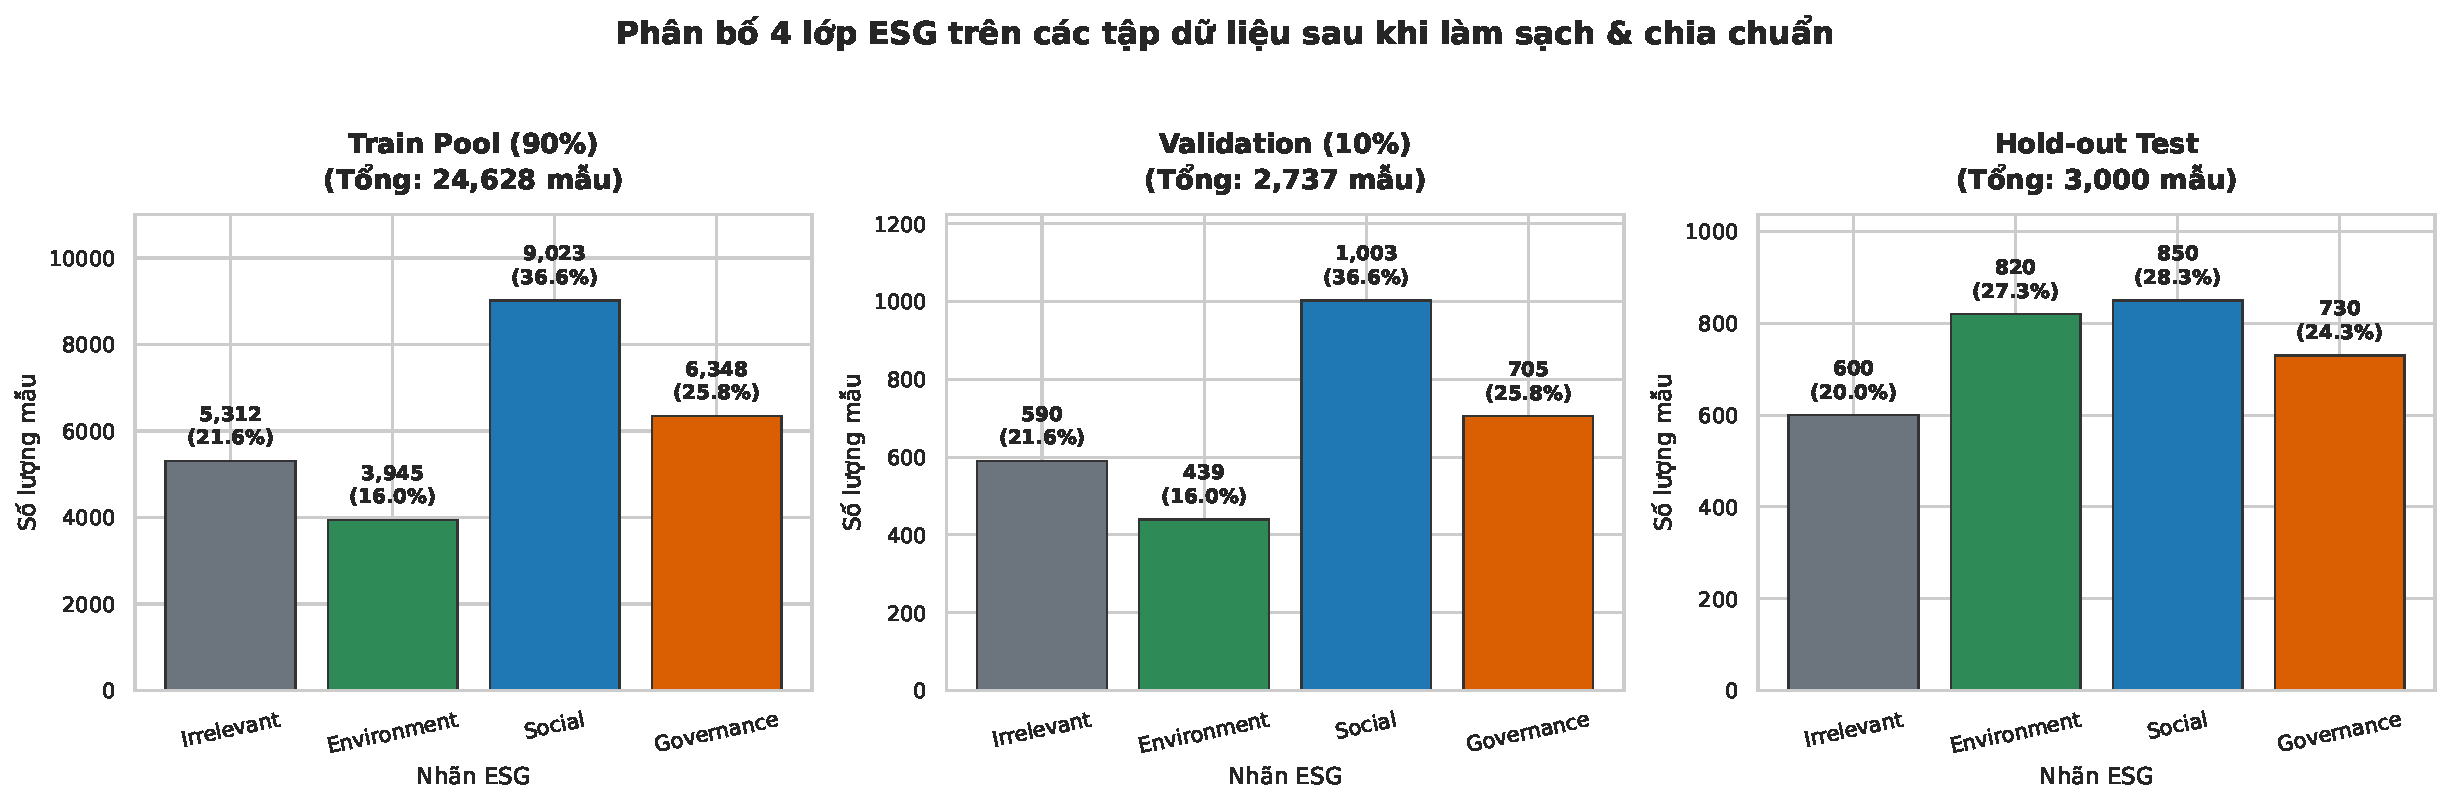
\includegraphics[width=0.92\textwidth]{B2_01_phan_bo_lop_esg.pdf}
  \caption{Phân bố bốn lớp ESG trên tập huấn luyện gốc, tập kiểm định và tập kiểm thử khóa kín, thể hiện dịch chuyển tỷ trọng ở lớp Environment ($+11{,}31\%$) và Social ($-8{,}31\%$).}
  \label{fig:eda_dist}
\end{figure*}

\begin{figure*}[!t]
  \centering
  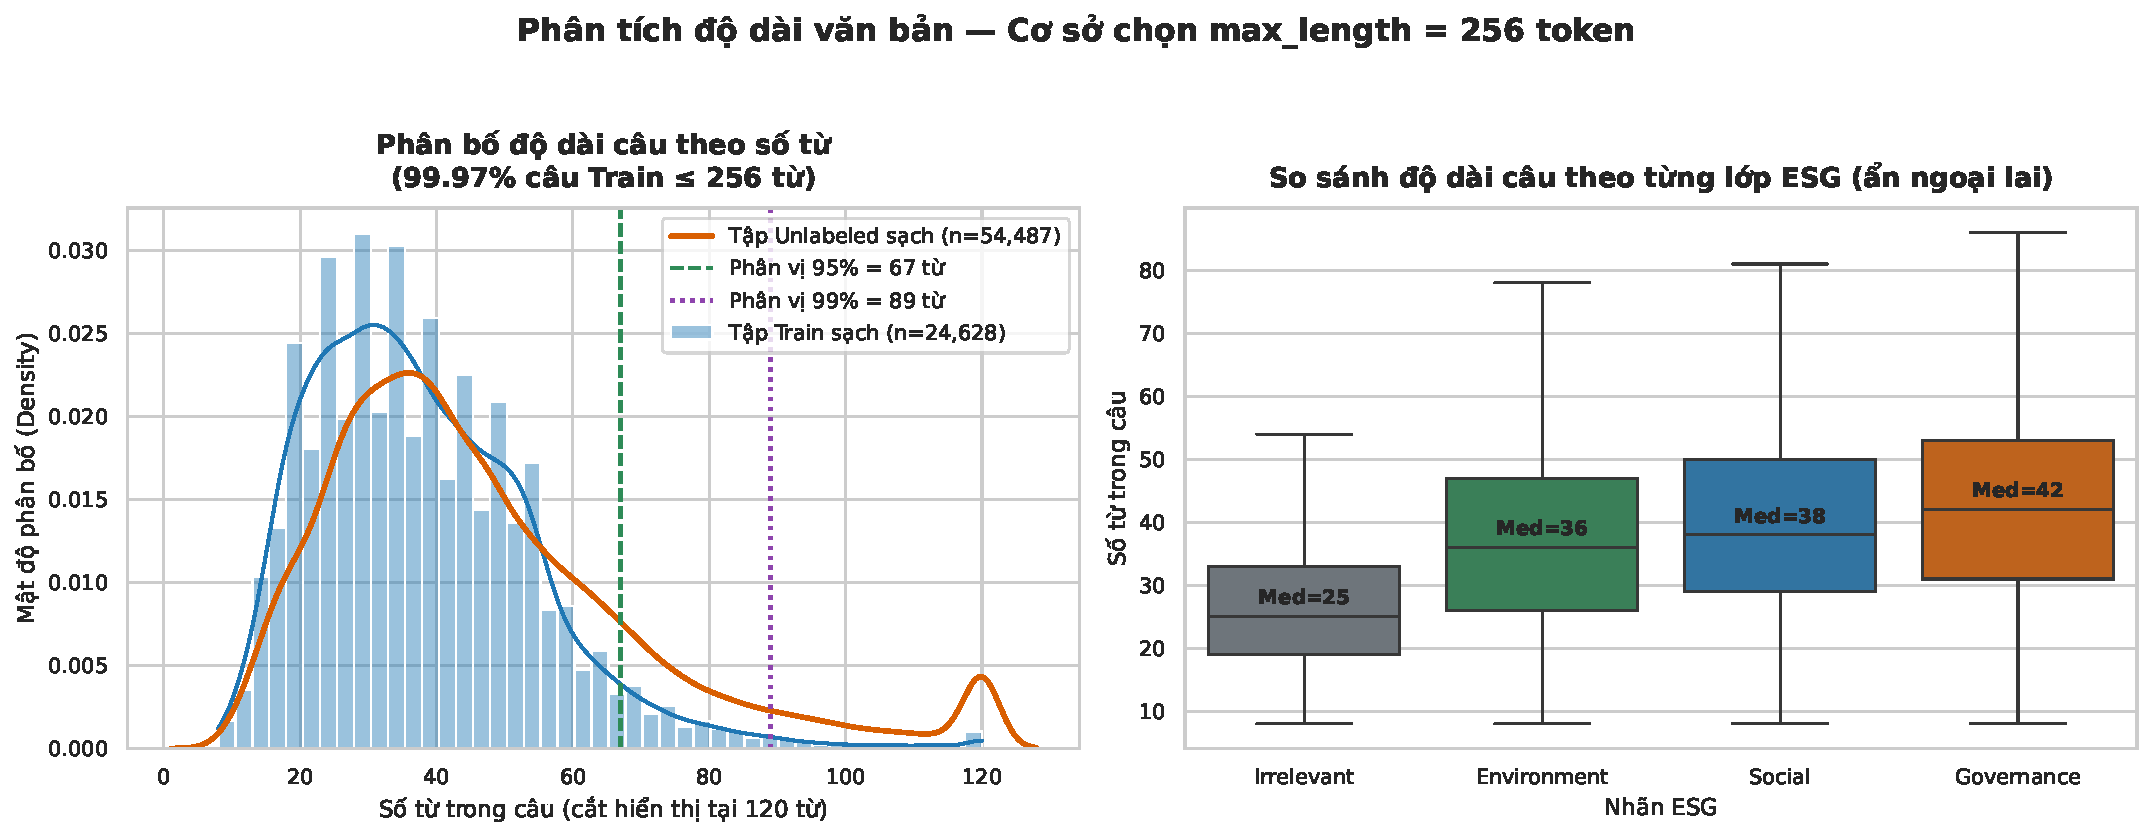
\includegraphics[width=0.95\textwidth]{B2_02_phan_bo_do_dai_van_ban.pdf}
  \caption{Phân bố độ dài câu giữa các miền dữ liệu (dịch chuyển độ dài câu) và phân tầng độ dài theo bốn lớp ESG.}
  \label{fig:eda_len}
\end{figure*}

\begin{figure*}[!t]
  \centering
  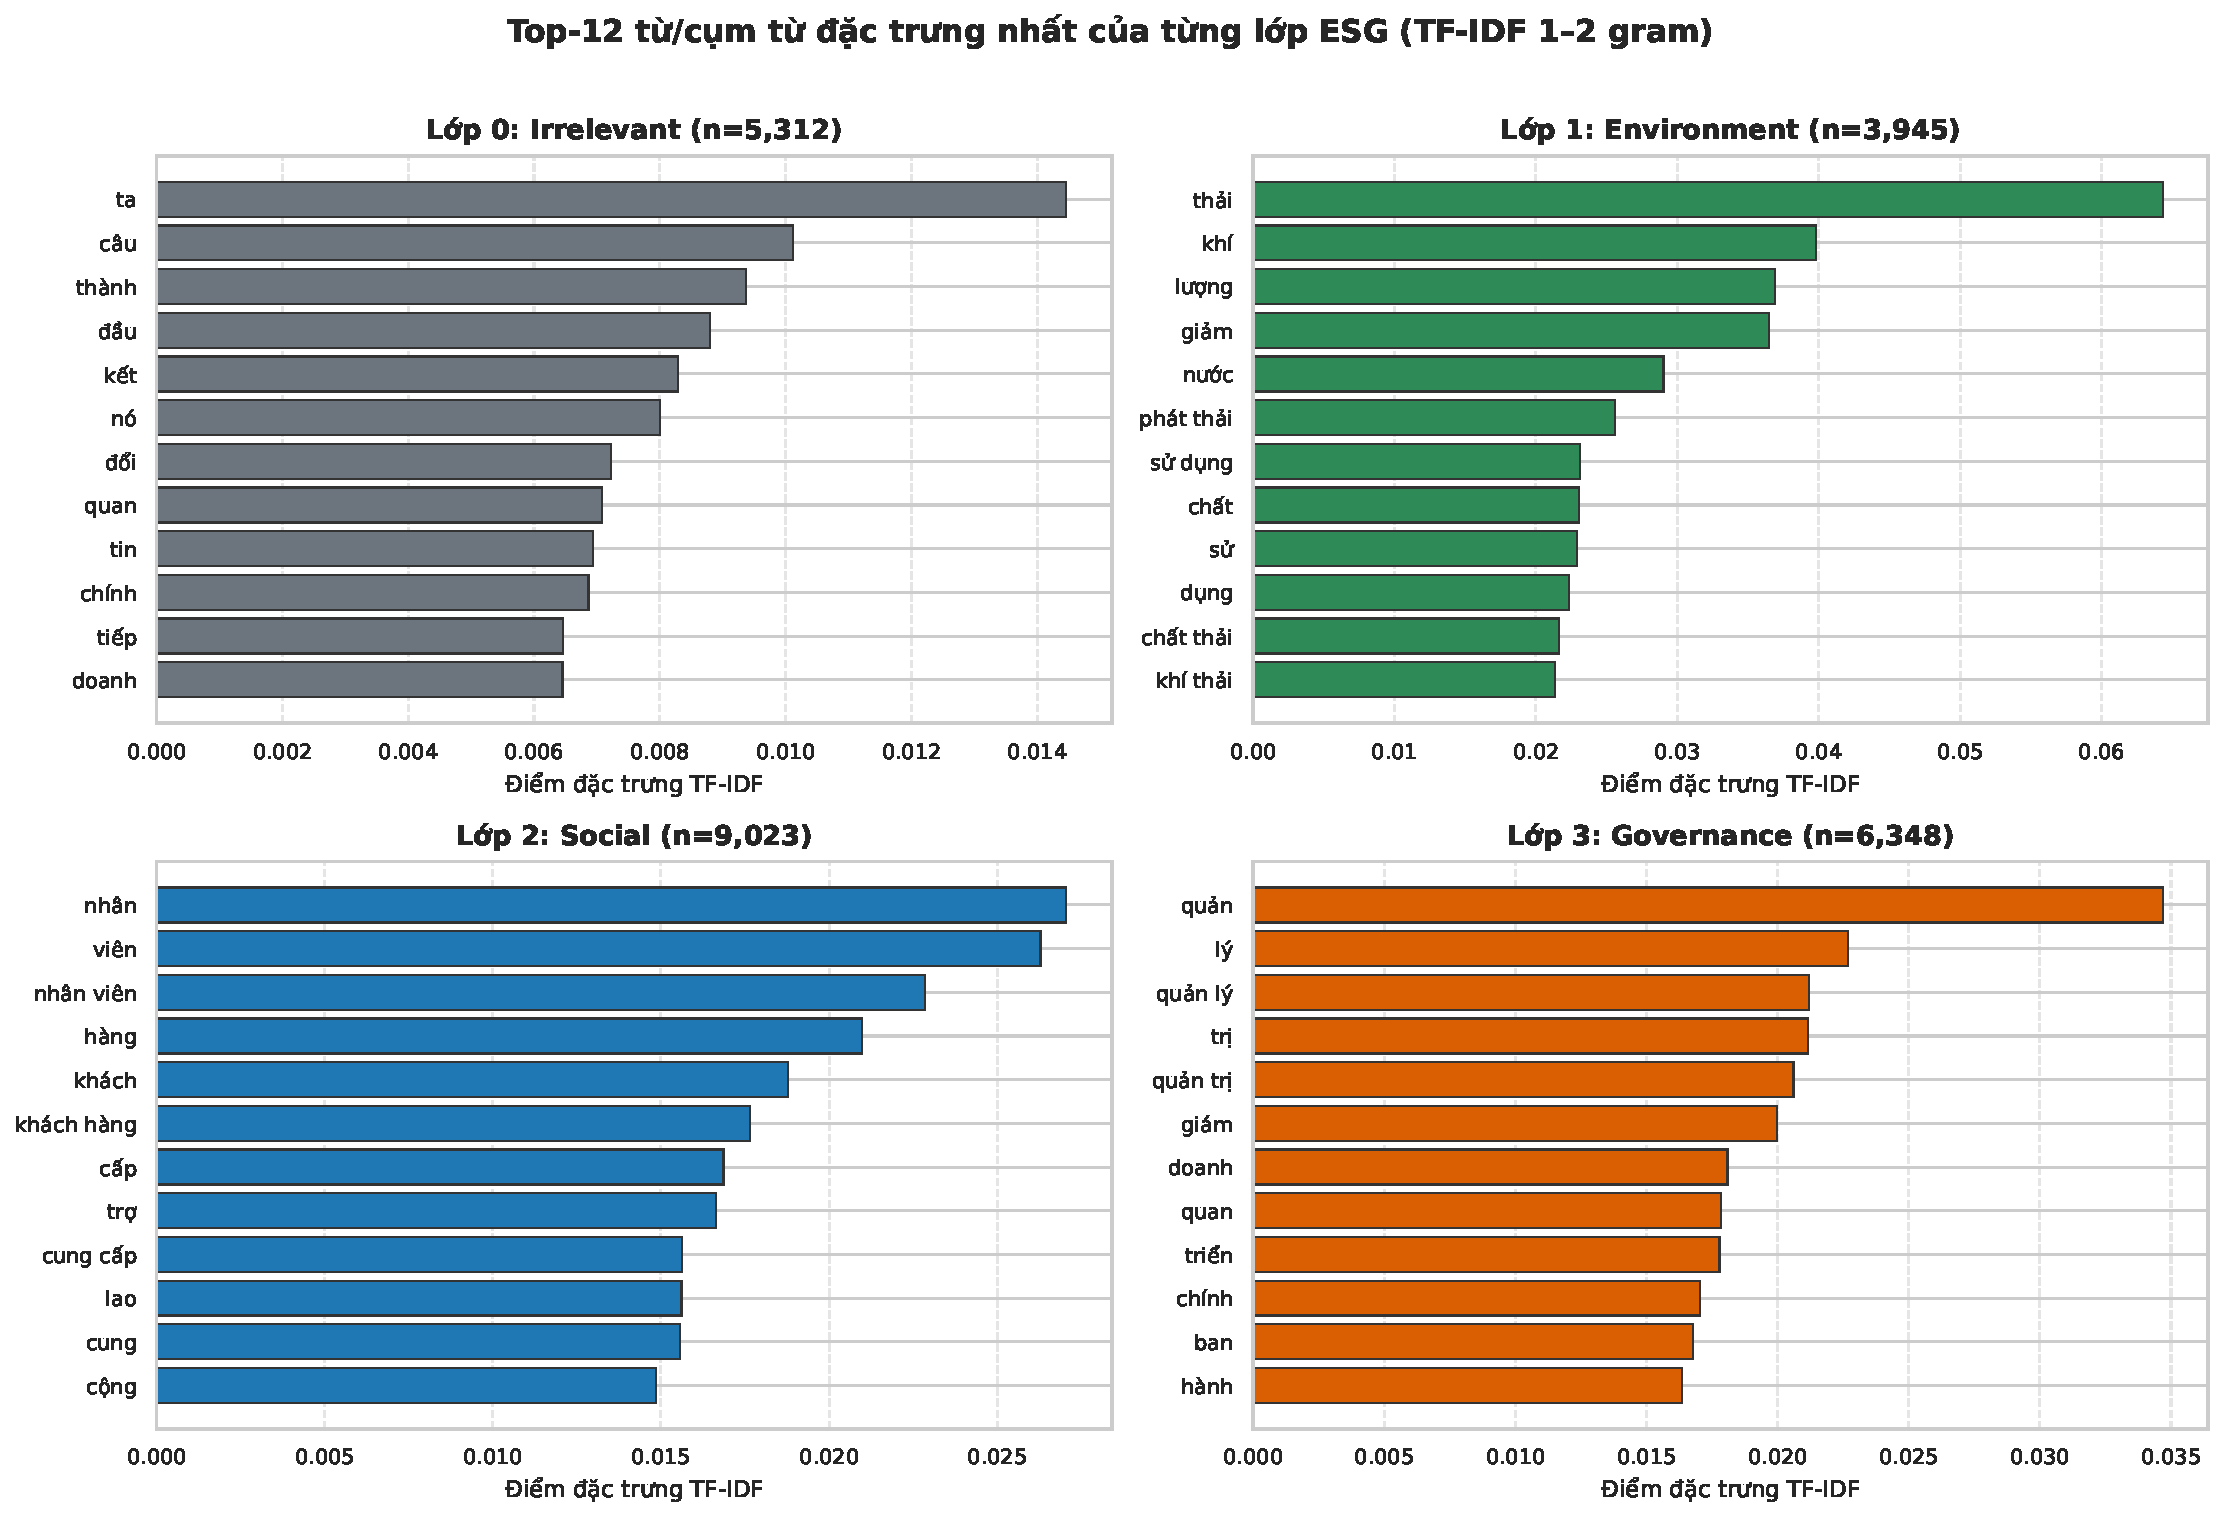
\includegraphics[width=0.92\textwidth]{B2_03_tu_khoa_dac_trung_4_lop.pdf}
  \caption{Mười hai từ và cụm từ đặc trưng có điểm TF-IDF cao nhất của từng lớp ESG.}
  \label{fig:eda_tfidf}
\end{figure*}

% ============================================================================
\section{Kết quả thực nghiệm}
\label{sec:results}

\subsection{Đối chứng Baseline, vòng~1 và phân tích lỗi nạp FP16 trên Transformers v5}

Kết quả huấn luyện đối chứng Baseline (trên 100\% \code{train\_pool}) và vòng~1 (trên bảy tập con 10.000 mẫu) được trình bày trong Bảng~\ref{tab:all_rounds}. Hai quan sát thực nghiệm đáng lưu ý gồm:

\textbf{Hiện tượng lệch hiệu chuẩn ở huấn luyện có giám sát thuần túy:} Mặc dù được huấn luyện trên lượng dữ liệu gấp 2,46 lần vòng~1, \code{Vi-ELECTRA Baseline} (Test Macro-F1 = 85,81\%, ECE = 0,1157) đạt hiệu năng kiểm thử thấp hơn \code{Vi-ELECTRA} vòng~1 dừng sớm ở epoch~3 (87,29\%, ECE = 0,0576). Hình~\ref{fig:lc_base} cho thấy từ epoch~3 trở đi, mất mát huấn luyện tiếp tục giảm dưới 0,10 trong khi mất mát kiểm định tăng trở lại ($0{,}35 \rightarrow 0{,}70$), phản ánh hiện tượng quá tự tin và khớp sát vào phân phối mất cân bằng ($IR=2{,}29$) của tập huấn luyện gốc~\cite{guo2017calibration}.

\begin{figure*}[!t]
  \centering
  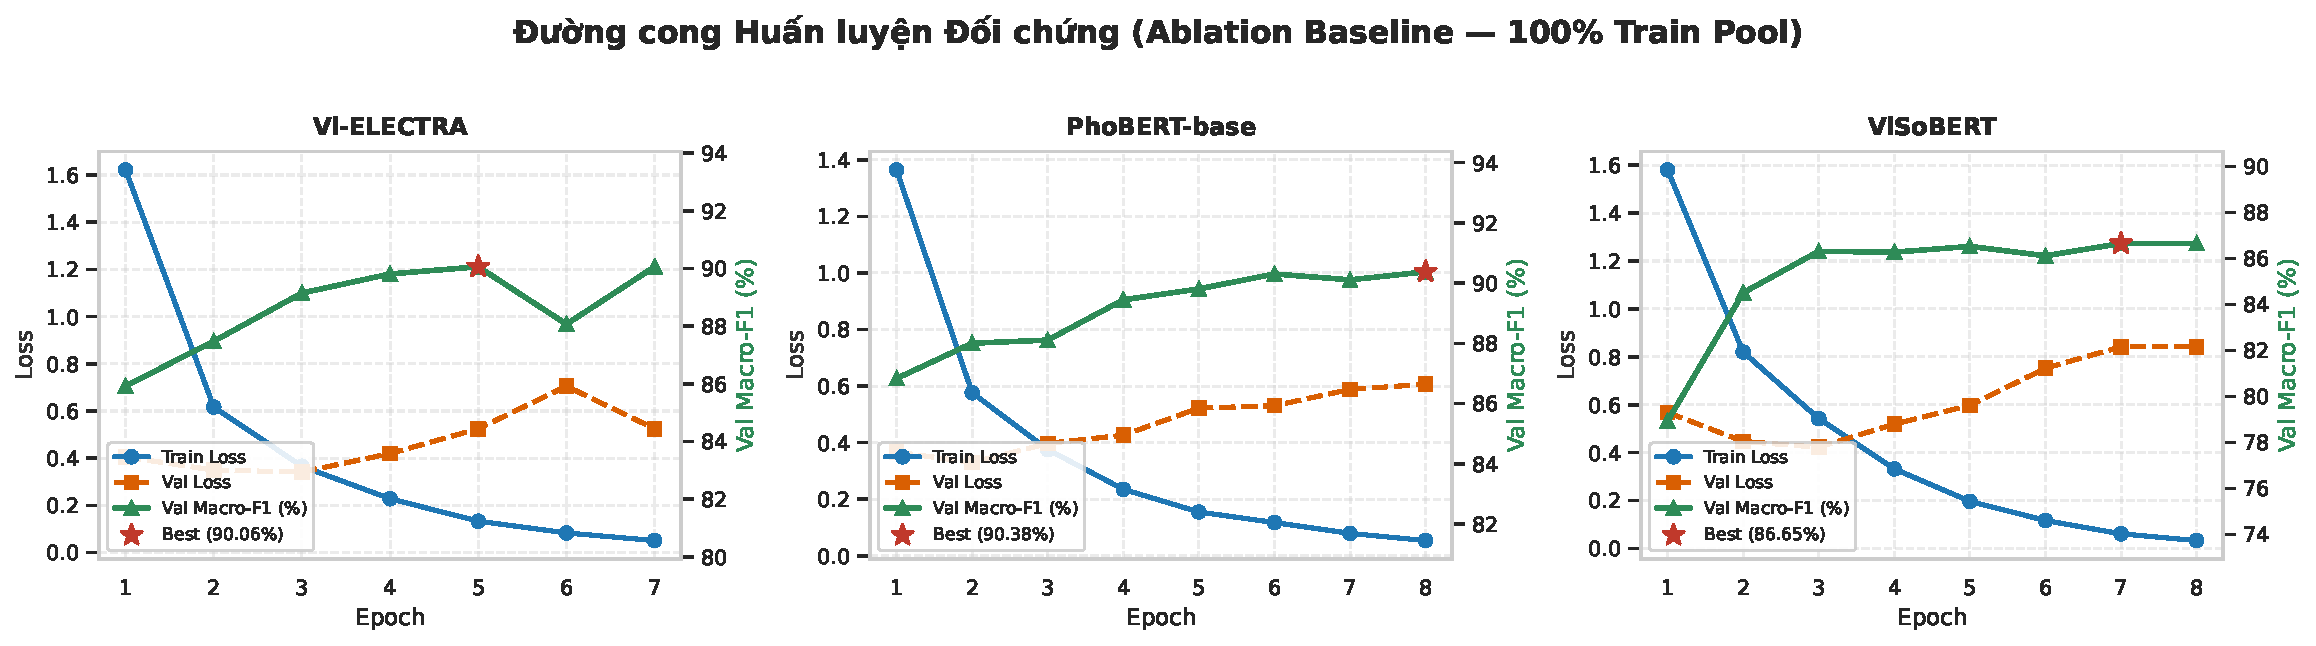
\includegraphics[width=0.96\textwidth]{B3_01b_learning_curves_baseline.pdf}
  \caption{Đường cong huấn luyện của ba mô hình đối chứng Baseline (100\% \code{train\_pool}), cho thấy xu hướng tăng mất mát kiểm định sau epoch~3.}
  \label{fig:lc_base}
\end{figure*}

\textbf{Phân tích và khắc phục lỗi suy biến của \code{ViDeBERTa-base}:} Tại vòng~1, \code{ViDeBERTa-base} hội tụ về trạng thái dự đoán toàn bộ sang lớp đa số \textit{Social} (Macro-F1 = 11,04\%). Kiểm tra cấu hình mô hình cho thấy kho \code{Fsoft-AIC/videberta-base} khai báo \code{torch\_dtype = float16} trong \code{config.json}; phiên bản \code{transformers 5.24.0} nạp trực tiếp tham số gốc ở định dạng \code{float16} thay vì \code{float32}, làm bước cập nhật AdamW (\code{lr=1.5e-5}) bị tràn dưới (\textit{underflow}) về~0. Việc chỉ định tường minh \code{dtype=torch.float32} nhằm duy trì trọng số gốc FP32 kết hợp tính toán hỗn hợp \code{BF16} và \code{activation\_checkpointing=True} đã khắc phục hoàn toàn hiện tượng này từ vòng~2 trở đi (\code{ViDeBERTa-base} đạt 83,75\% ở vòng~2 và 85,14\% ở vòng~3, mức VRAM đỉnh 3,17--3,36~GB).

\subsection{Chất lượng gán nhãn giả qua hai vòng và hiệu chỉnh dịch chuyển tiên nghiệm}

\begin{figure*}[!t]
  \centering
  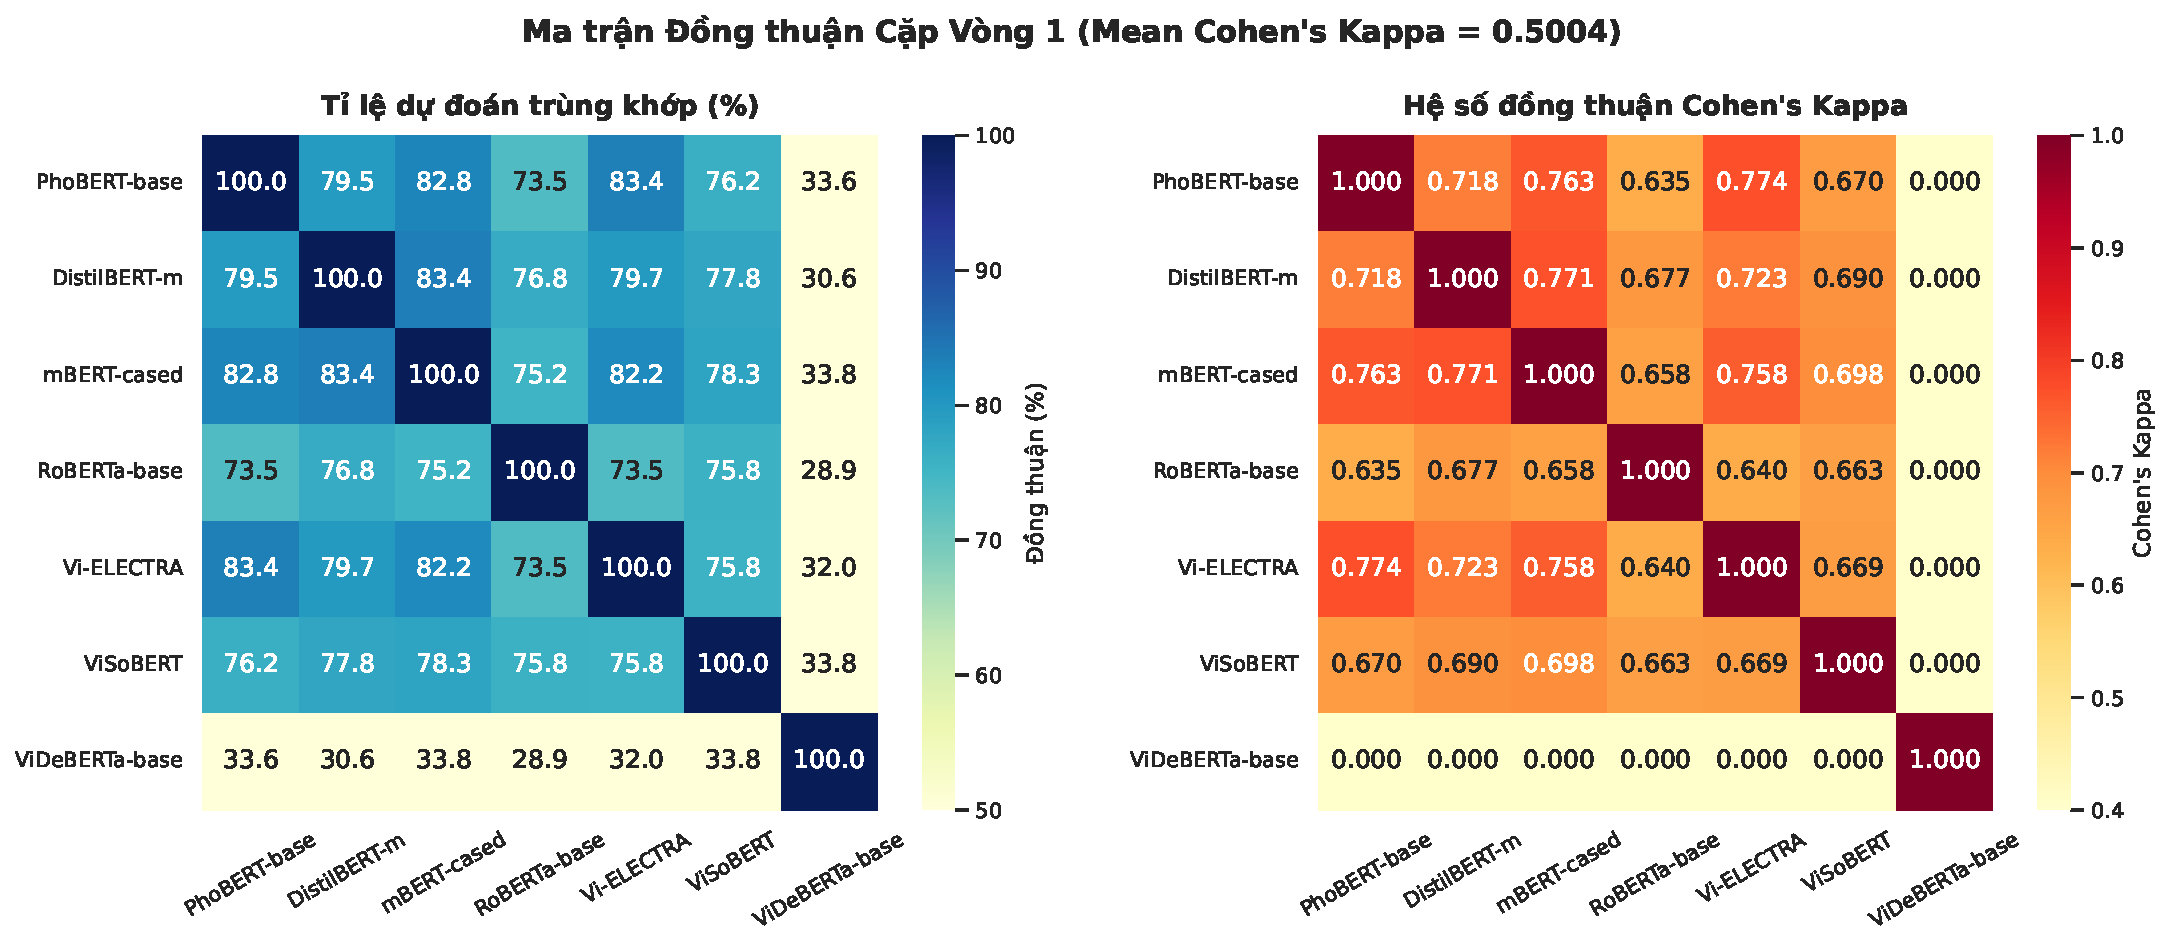
\includegraphics[width=0.95\textwidth]{B4_02_ma_tran_dong_thuan_kappa.pdf}
  \caption{Ma trận đồng thuận cặp (\%) và hệ số Cohen's Kappa ở vòng~1 giữa bảy mô hình (sáu mô hình hội tụ đạt $\kappa \in [0{,}635; 0{,}774]$).}
  \label{fig:kappa_r1}
\end{figure*}

\begin{figure*}[!t]
  \centering
  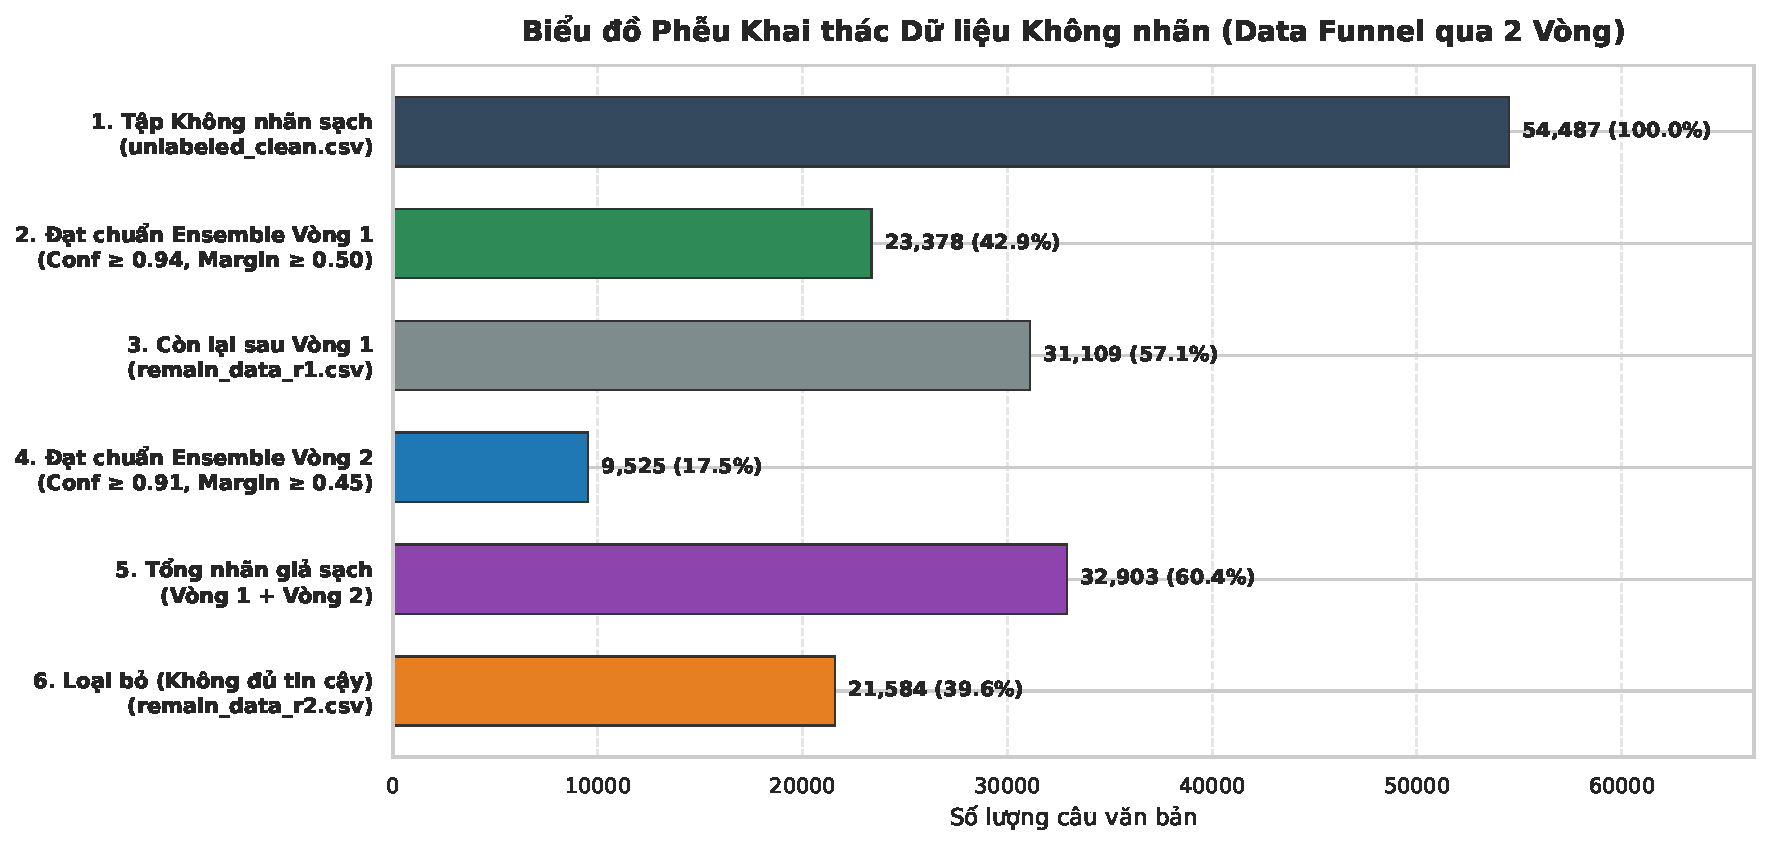
\includegraphics[width=0.88\textwidth]{B6_01_bieu_do_pheu_unlabeled.pdf}
  \caption{Biểu đồ phễu theo dõi quá trình khai thác 54.487 câu không nhãn qua hai vòng đồng thuận: giữ lại 32.903 mẫu (60,4\%) và loại bỏ 21.584 mẫu bất định (39,6\%).}
  \label{fig:funnel}
\end{figure*}

\begin{figure*}[!t]
  \centering
  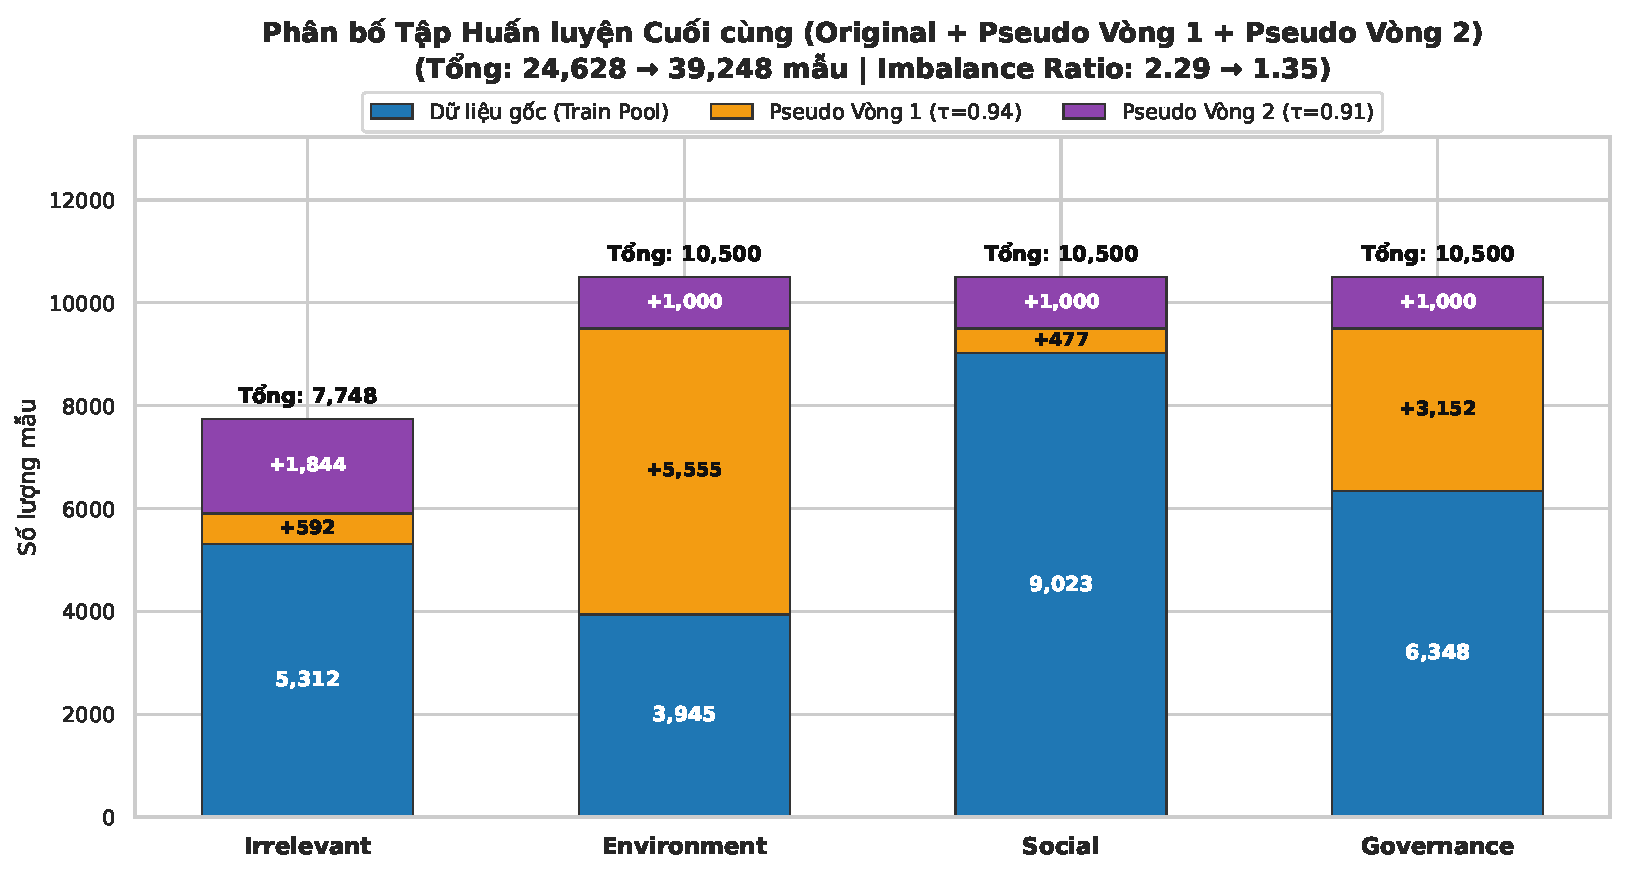
\includegraphics[width=0.85\textwidth]{B6_02_phan_bo_du_lieu_3_tang.pdf}
  \caption{Phân bố bốn lớp ESG của tập huấn luyện cuối cùng (39.248 mẫu) sau hai vòng bổ sung nhãn giả, đưa $IR$ từ $2{,}29$ xuống $1{,}35$.}
  \label{fig:stacked3}
\end{figure*}

\begin{figure*}[!t]
  \centering
  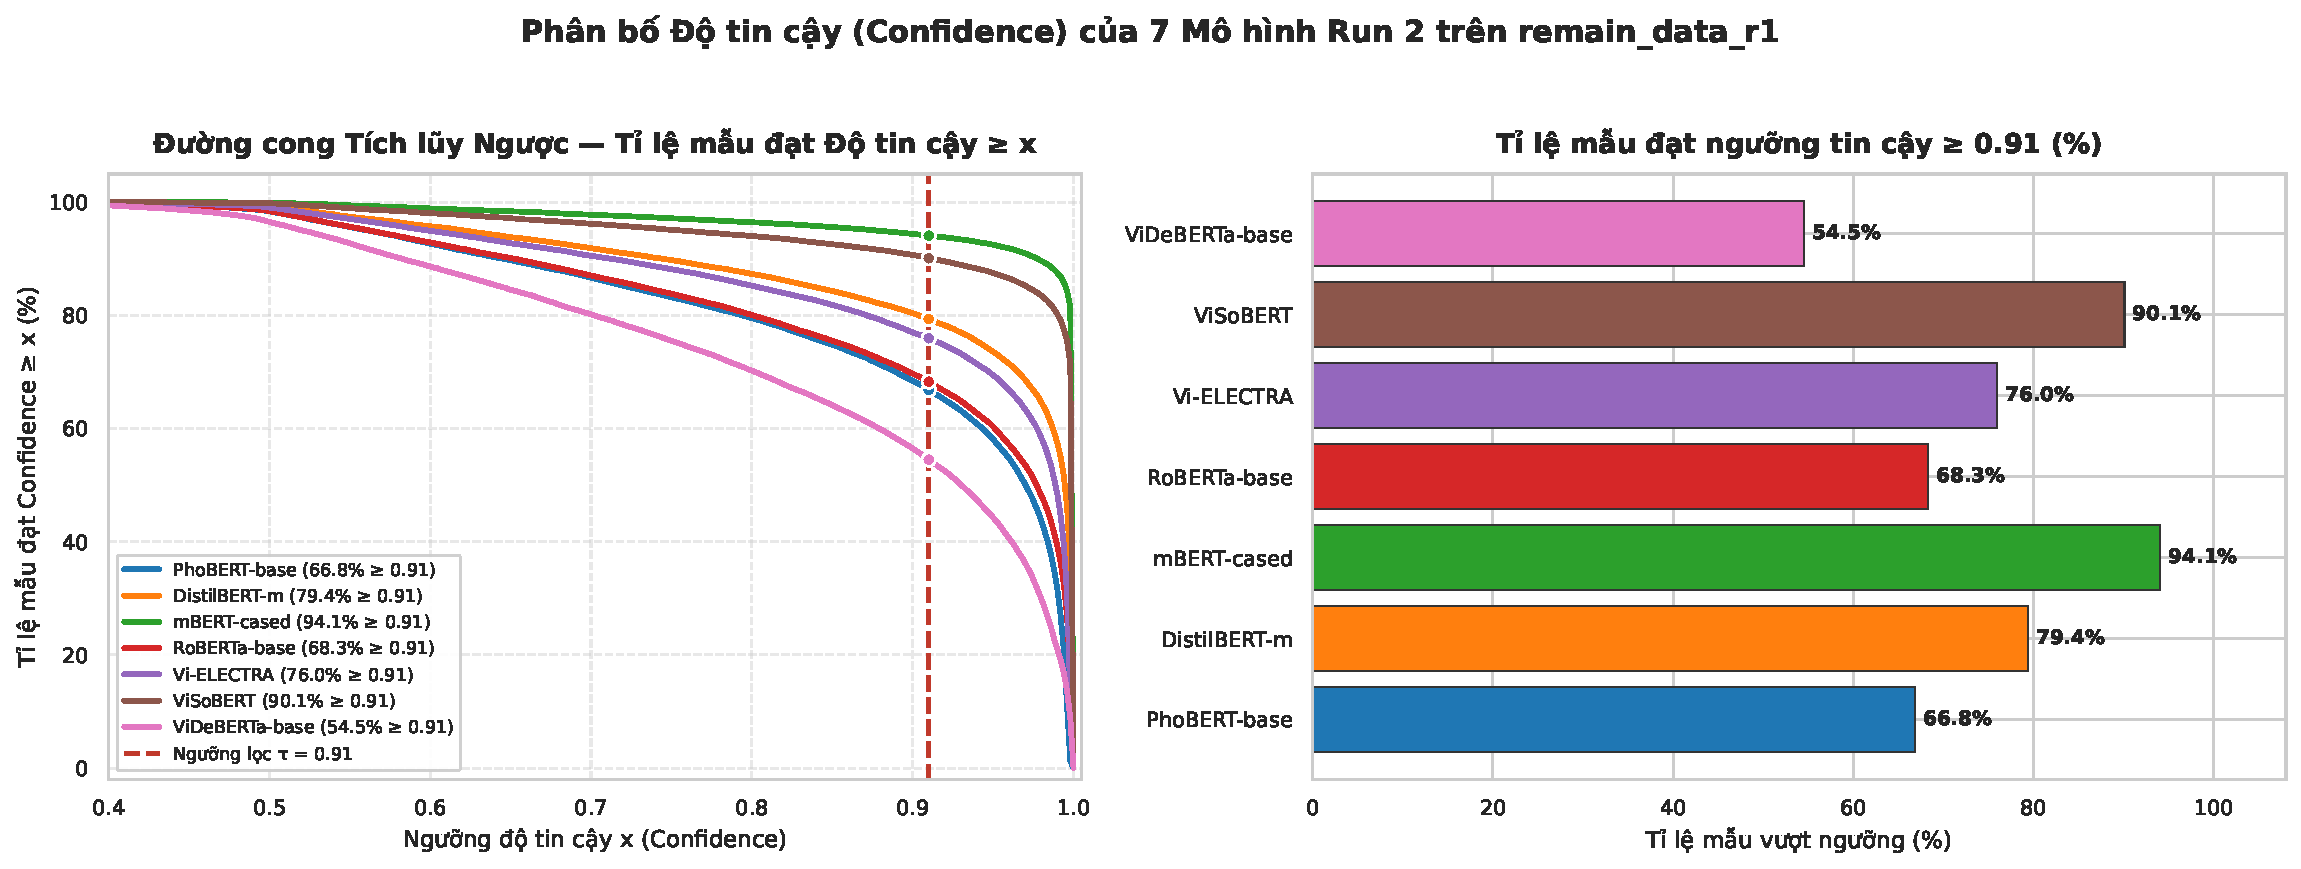
\includegraphics[width=0.86\textwidth]{B6_03_phan_bo_confidence_vong2.pdf}
  \caption{Đường cong tích lũy ngược độ tin cậy ($1-\text{ECDF}$) của bảy mô hình vòng~2 trên 31.109 câu còn lại sau vòng~1 (\code{remain\_data\_r1.csv}).}
  \label{fig:ecdf_r2}
\end{figure*}

Ở vòng~1, sáu mô hình hội tụ đạt mức đồng thuận cặp $73{,}5\%\text{--}83{,}4\%$ với hệ số Cohen's Kappa trung bình $\bar{\kappa} = 0{,}706$, tương ứng mức đồng thuận khá tốt (\textit{Substantial Agreement}) theo thang phân loại của Landis và Koch~\cite{landis1977measurement} (Hình~\ref{fig:kappa_r1}). Nhờ cơ chế gán trọng số tỷ lệ theo \code{Val Macro-F1}, \code{ViDeBERTa-base} chỉ nhận trọng số 2,53\%, hạn chế ảnh hưởng lên 23.378 nhãn giả được tuyển chọn (độ tin cậy trung bình 0,9682, biên độ trung bình 0,9533). Tuy nhiên, do ngưỡng lọc vòng~1 cao ($\tau_1=0{,}94$), lớp \textit{Irrelevant} chỉ bổ sung được 592 mẫu (tổng 5.904 mẫu so với 9.500 mẫu của ba lớp E--S--G), là nguyên nhân khiến \code{PhoBERT-base} và \code{Vi-ELECTRA} giảm nhẹ khoảng 0,5 điểm phần trăm trên tập kiểm thử ở vòng~2 dù tăng điểm trên tập kiểm định.

Ở vòng~2, cả bảy mô hình vòng~2 đều hội tụ với trọng số phân bố đều ($0{,}1365\text{--}0{,}1477$) và tuyển chọn thêm 9.525 mẫu từ 31.109 câu còn lại, trong đó 9.289/9.525 mẫu (97,52\%) đạt đồng thuận 7/7 mô hình (độ tin cậy trung bình 0,9738, entropy trung bình 0,1205). Đường cong tích lũy ngược $1-\text{ECDF}$ ở Hình~\ref{fig:ecdf_r2} phản ánh sự bổ trợ về mức độ tự tin giữa các kiến trúc: \code{mBERT-cased} và \code{ViSoBERT} có tỷ lệ vượt ngưỡng $\ge 0{,}91$ trên 90\%, trong khi \code{ViDeBERTa-base} (54,5\%) và \code{PhoBERT-base} (66,8\%) có xu hướng thận trọng hơn, hỗ trợ hạn chế hiện tượng quá tự tin khi tổng hợp xác suất. Tổng hợp hai vòng (Hình~\ref{fig:funnel} và Hình~\ref{fig:stacked3}), hệ thống sử dụng 32.903/54.487 câu không nhãn (60,4\%), nâng lớp \textit{Irrelevant} lên 7.748 mẫu (19,74\%, xấp xỉ mức 20,00\% của tập kiểm thử) và đưa ba lớp E--S--G lên 10.500 mẫu mỗi lớp (26,75\%), kéo tỷ số mất cân bằng $IR$ giảm từ $2{,}29 \rightarrow 1{,}61 \rightarrow 1{,}35$.

\subsection{Kết quả vòng~3, hệ thống Ensemble cuối cùng và kiểm định McNemar}

\begin{table*}[!t]
\centering
\caption{Tổng hợp hiệu năng của bảy mô hình đơn lẻ (vòng~3 trên 39.248 mẫu) và bốn chiến lược kết hợp Ensemble trên tập kiểm thử khóa kín (3.000 mẫu), kèm sai số hiệu chuẩn ECE và tốc độ suy luận trên RTX 5070.}
\label{tab:run3_ens}
\footnotesize
\renewcommand{\arraystretch}{1.15}
\setlength{\tabcolsep}{3.5pt}
\begin{adjustbox}{max width=\textwidth}
\begin{tabular}{@{}lccccccccccccc@{}}
\toprule
\textbf{Mô hình / Chiến lược} & \textbf{Ep} & \textbf{Val F1} & \textbf{Test Acc} & \textbf{Macro-F1} & \textbf{$\Delta$ F1} & \textbf{F1 Irr} & \textbf{F1 Env} & \textbf{F1 Soc} & \textbf{F1 Gov} & \textbf{ECE $\downarrow$} & \textbf{ms/câu} & \textbf{mẫu/s} & \textbf{VRAM} \\
\midrule
\textbf{DistilBERT-m} \textit{(đơn lẻ tốt nhất)} & 4 & 89,37 & \best{89,70} & \best{89,03} & \best{$+$3,23} & \best{79,87} & 97,77 & 88,21 & \best{90,26} & \best{0,0825} & \best{0,324} & \best{3.085} & 2,96 GB \\
mBERT-cased & 6 & 89,82 & 89,43 & 88,48 & $+$1,56 & 78,92 & 96,89 & \best{89,54} & 88,58 & 0,0988 & 0,550 & 1.818 & 4,47 GB \\
PhoBERT-base & 5 & \best{91,10} & 88,97 & 88,13 & $+$2,24 & 78,41 & \best{97,88} & 88,16 & 88,08 & 0,1018 & 0,493 & 2.028 & 3,86 GB \\
ViSoBERT & 8 & 87,64 & 88,30 & 87,49 & $+$2,51 & 78,69 & 97,09 & 87,98 & 86,22 & 0,1117 & 0,601 & 1.663 & 3,30 GB \\
Vi-ELECTRA & 4 & 90,55 & 88,23 & 87,31 & $+$0,52 & 77,41 & 97,47 & 87,43 & 86,92 & 0,1055 & 0,495 & 2.019 & 3,83 GB \\
RoBERTa-base & 6 & 85,26 & 88,13 & 86,95 & $+$2,46 & 75,61 & 95,86 & 89,28 & 87,04 & 0,0898 & 0,977 & 1.024 & 3,70 GB \\
ViDeBERTa-base & 6 & 83,55 & 86,17 & 85,14 & $+$1,39 & 74,38 & 95,16 & 85,47 & 85,56 & 0,0864 & 0,834 & 1.199 & 3,36 GB \\
\midrule
\textbf{Ensemble -- Equal Soft (7M)} & --- & --- & \best{90,77} & \best{90,09} & --- & \best{82,54} & \best{98,18} & \best{90,39} & 89,24 & \best{0,0226} & 4,274 & 234 & --- \\
Ensemble -- Weighted Soft (7M) & --- & --- & 90,73 & 90,04 & --- & 82,36 & 98,12 & \best{90,39} & \best{89,29} & 0,0256 & 4,274 & 234 & --- \\
Ensemble -- Hard Voting (7M) & --- & --- & 90,63 & 89,95 & --- & 82,36 & 98,12 & 90,20 & 89,11 & 0,0290 & 4,274 & 234 & --- \\
Ensemble -- Top-3 Weighted & --- & --- & 89,90 & 89,08 & --- & 80,14 & 98,01 & 89,52 & 88,64 & 0,0589 & 1,538 & 650 & --- \\
\bottomrule
\multicolumn{14}{@{}l@{}}{\scriptsize Ghi chú: Cột $\Delta$ F1 biểu thị chênh lệch Macro-F1 giữa vòng~3 và vòng~2 trên tập kiểm thử khóa kín.}
\end{tabular}
\end{adjustbox}
\end{table*}

\begin{table*}[!t]
\centering
\caption{Diễn tiến Macro-F1 (\%) và Accuracy (\%) trong ngoặc đơn qua các giai đoạn từ đối chứng Baseline, ba vòng huấn luyện đến mô hình Ensemble cuối cùng trên tập kiểm thử.}
\label{tab:all_rounds}
\footnotesize
\renewcommand{\arraystretch}{1.15}
\setlength{\tabcolsep}{5pt}
\begin{adjustbox}{max width=\textwidth}
\begin{tabular}{@{}lcccccc@{}}
\toprule
\textbf{Mô hình / Hệ thống} & \textbf{Baseline (24,6k)} & \textbf{Vòng 1 (10k)} & \textbf{Vòng 2 (34,4k)} & \textbf{Vòng 3 (39,2k)} & \textbf{$\Delta$ (V3 $-$ Base)} & \textbf{$\Delta$ (V3 $-$ V1)} \\
\midrule
PhoBERT-base & 86,46 (87,80) & 86,43 (87,67) & 85,89 (87,27) & \best{88,13} (88,97) & \best{$+$1,67} & $+$1,70 \\
Vi-ELECTRA & 85,81 (87,07) & 87,29 (88,03) & 86,79 (87,77) & \best{87,31} (88,23) & \best{$+$1,50} & $+$0,02 \\
ViSoBERT & 82,93 (84,73) & 80,37 (82,90) & 84,98 (85,77) & \best{87,49} (88,30) & \best{$+$4,56} & \best{$+$7,12} \\
DistilBERT-m & --- & 83,86 (85,37) & 85,80 (87,10) & \best{89,03} (89,70) & --- & \best{$+$5,17} \\
mBERT-cased & --- & 86,06 (87,60) & 86,92 (88,00) & \best{88,48} (89,43) & --- & $+$2,42 \\
RoBERTa-base & --- & 79,28 (81,33) & 84,49 (86,00) & \best{86,95} (88,13) & --- & \best{$+$7,67} \\
ViDeBERTa-base & --- & 11,04\textsuperscript{$\ddagger$} (28,33) & 83,75 (84,90) & \best{85,14} (86,17) & --- & Khôi phục \\
\midrule
\textbf{Equal Soft Ensemble (7M)} & --- & --- & --- & \best{90,09 (90,77)} & \best{$+$3,63}\textsuperscript{*} & \best{$+$2,80}\textsuperscript{$\dagger$} \\
\bottomrule
\multicolumn{7}{@{}l@{}}{\scriptsize \textsuperscript{*}So với Baseline cao nhất (\code{PhoBERT-base}: 86,46\% / 87,80\%). \textsuperscript{$\dagger$}So với vòng~1 cao nhất (\code{Vi-ELECTRA}: 87,29\% / 88,03\%). \textsuperscript{$\ddagger$}Suy biến do lỗi nạp FP16.}
\end{tabular}
\end{adjustbox}
\end{table*}

\begin{table}[!t]
\centering
\caption{Kết quả kiểm định ý nghĩa thống kê McNemar ($\alpha = 0{,}05$) trên 3.000 mẫu kiểm thử.}
\label{tab:mcnemar}
\footnotesize
\renewcommand{\arraystretch}{1.15}
\setlength{\tabcolsep}{3.5pt}
\begin{adjustbox}{max width=\columnwidth}
\begin{tabular}{@{}lccccc@{}}
\toprule
\textbf{So sánh Equal Soft (7M) với} & \textbf{$n_{10}$} & \textbf{$n_{01}$} & \textbf{Ròng} & \textbf{$\chi^2$} & \textbf{$p$-value} \\
\midrule
Đơn lẻ tốt nhất (\code{DistilBERT-m}) & 99 & 67 & $+$32 & 5,789 & \best{0,0161} \\
Baseline tốt nhất (\code{PhoBERT-base}) & 162 & 73 & $+$89 & 32,953 & \best{$<10^{-6}$} \\
\bottomrule
\end{tabular}
\end{adjustbox}
\end{table}

\begin{figure*}[!t]
  \centering
  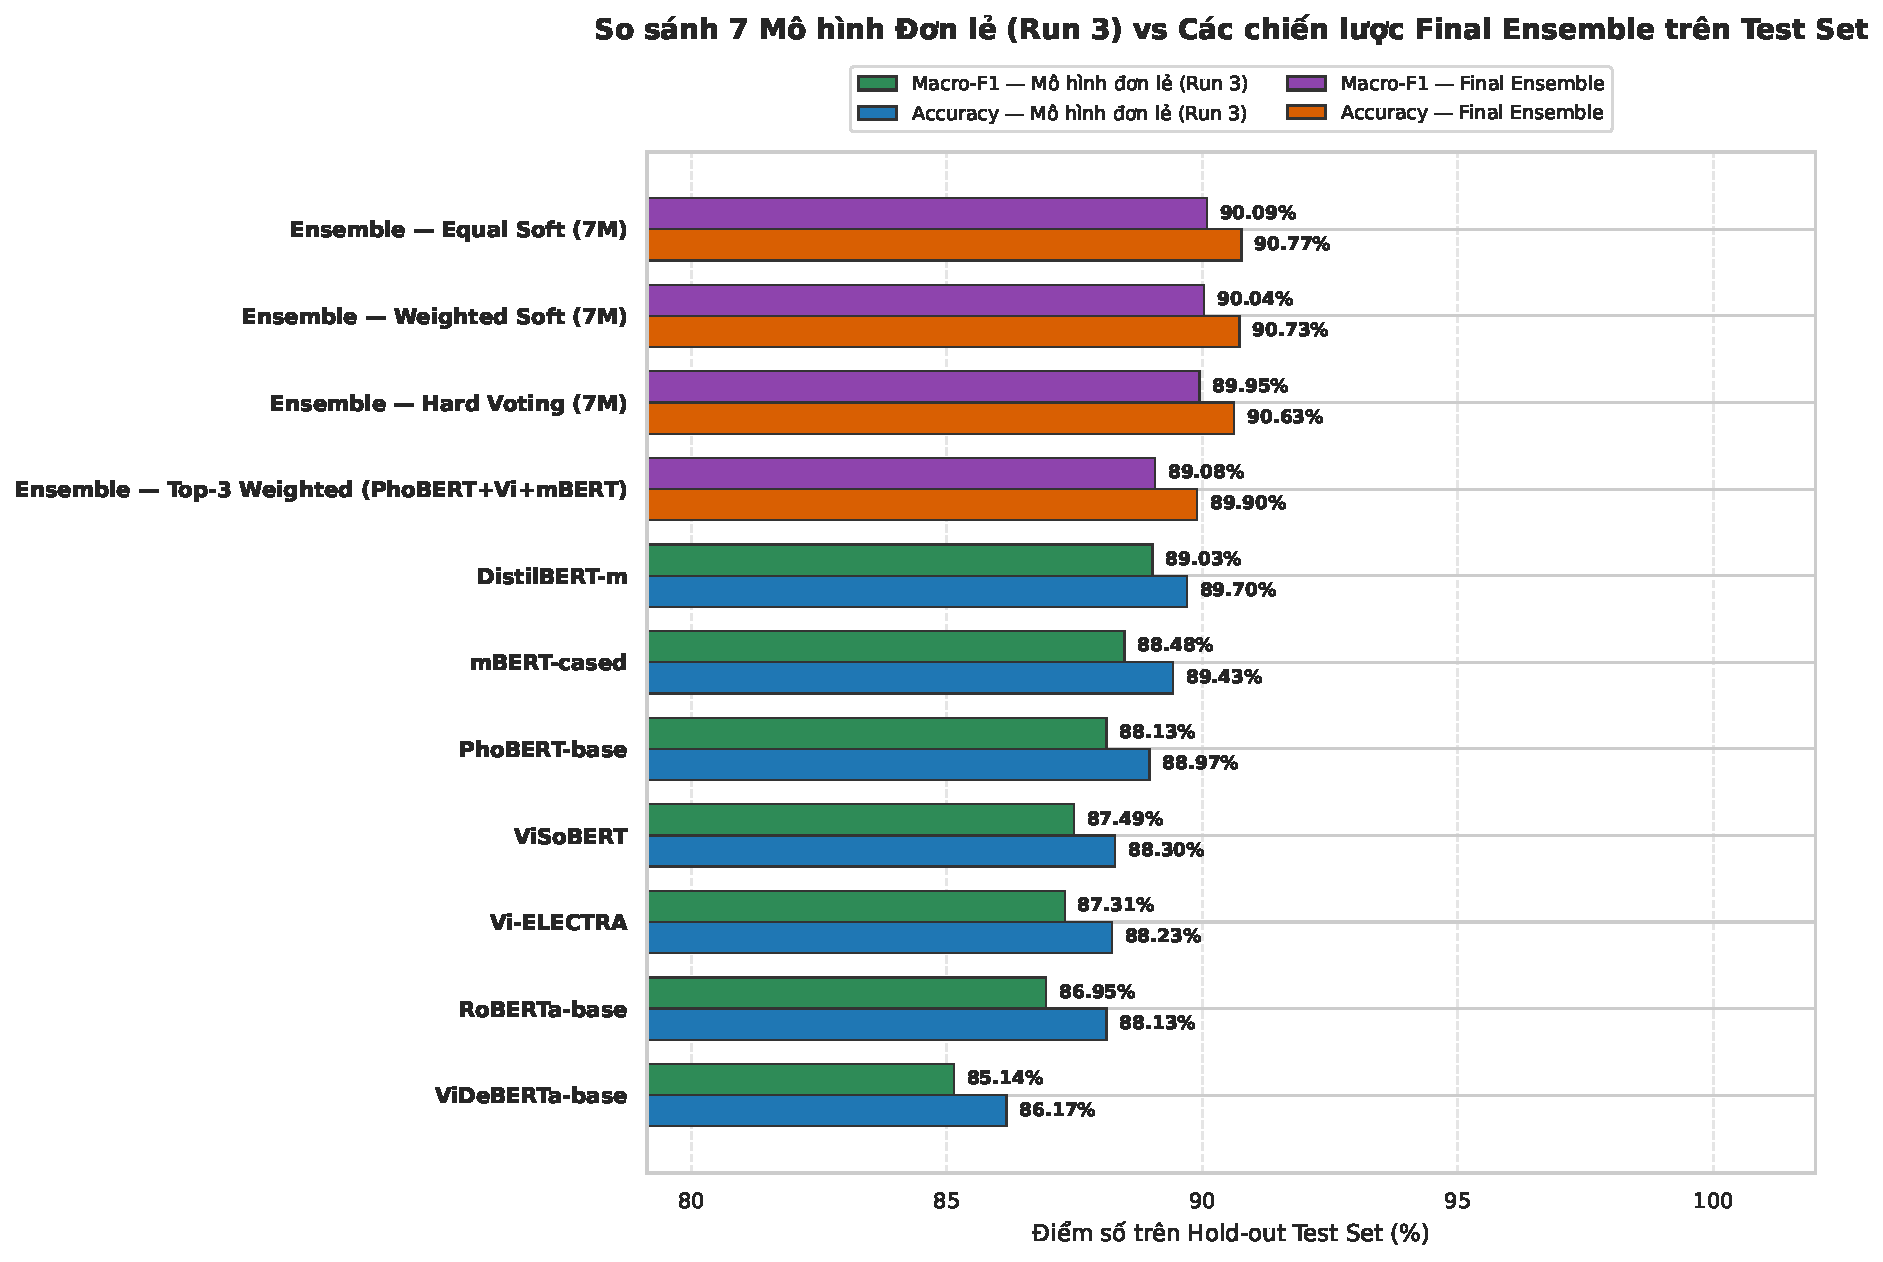
\includegraphics[width=0.92\textwidth]{B7_01_so_sanh_don_le_va_ensemble.pdf}
  \caption{So sánh Macro-F1 và Accuracy giữa bảy mô hình đơn lẻ (vòng~3) và bốn chiến lược kết hợp Ensemble trên tập kiểm thử khóa kín.}
  \label{fig:r3_ens}
\end{figure*}

Từ Bảng~\ref{tab:run3_ens}, Bảng~\ref{tab:all_rounds} và Hình~\ref{fig:r3_ens}, có bốn kết quả định lượng chính được rút ra:
\begin{enumerate}[leftmargin=*, itemsep=2pt, topsep=2pt]
  \item \textbf{Cải thiện đồng đều trên cả bảy mô hình ở vòng~3:} Sau khi bổ sung thêm 1.844 mẫu lớp \textit{Irrelevant} ở vòng~2, toàn bộ bảy mô hình đều tăng điểm so với vòng~2 ($+0{,}52\%$ đến $+3{,}23\%$ Macro-F1). Riêng F1 lớp \textit{Irrelevant} tăng $+6{,}52\%$ ở \code{PhoBERT-base} và $+6{,}40\%$ ở \code{DistilBERT-m}.
  \item \textbf{Kết quả thực nghiệm đối chứng (Hình~\ref{fig:progress}):} Cả ba kiến trúc tiếng Việt đều đạt Macro-F1 cao hơn ở vòng~3 so với bản huấn luyện có giám sát trên 100\% \code{train\_pool} gốc (\code{PhoBERT-base} $+1{,}67\%$, \code{Vi-ELECTRA} $+1{,}50\%$, \code{ViSoBERT} $+4{,}56\%$). Các mô hình có điểm xuất phát thấp hơn ở vòng~1 ghi nhận mức tăng lớn nhất (\code{RoBERTa-base} $+7{,}67\%$, \code{ViSoBERT} $+7{,}12\%$, \code{DistilBERT-m} $+5{,}17\%$), cho thấy tác dụng truyền tải tri thức gián tiếp thông qua nhãn giả đồng thuận.
  \item \textbf{Khả năng tổng quát hóa của \code{DistilBERT-m}:} Dù \code{PhoBERT-base} có điểm kiểm định cao nhất (91,10\%), \code{DistilBERT-m} (6 lớp) lại đạt điểm kiểm thử cao nhất trong nhóm đơn lẻ (89,03\% Macro-F1 / 89,70\% Accuracy). Độ chênh lệch giữa tập kiểm định và tập kiểm thử của \code{DistilBERT-m} là nhỏ nhất ($+0{,}34\%$ so với $+2{,}97\%$ ở \code{PhoBERT-base}), đi kèm sai số hiệu chuẩn thấp nhất nhóm đơn lẻ ($\text{ECE} = 0{,}0825$) và khả năng xử lý ổn định các câu có thuật ngữ tiếng Anh xen kẽ mà không phụ thuộc bộ tách từ \code{pyvi}.
  \item \textbf{Hiệu quả và ý nghĩa thống kê của Ensemble 7 mô hình:} Chiến lược trung bình xác suất đồng đều (\code{Equal Soft 7M}) đạt 90,77\% Accuracy và 90,09\% Macro-F1, cao hơn nhẹ so với \code{Weighted Soft 7M} (90,04\%) do trọng số $1/7$ tránh đặt tỷ trọng quá lớn vào các mô hình có độ chênh lệch Val--Test cao. Kiểm định McNemar (Bảng~\ref{tab:mcnemar}) xác nhận sự cải thiện này có ý nghĩa thống kê so với cả \code{DistilBERT-m} ($p = 0{,}0161 < 0{,}05$) và Baseline cao nhất ($p < 10^{-6}$).
\end{enumerate}

\begin{figure*}[!t]
  \centering
  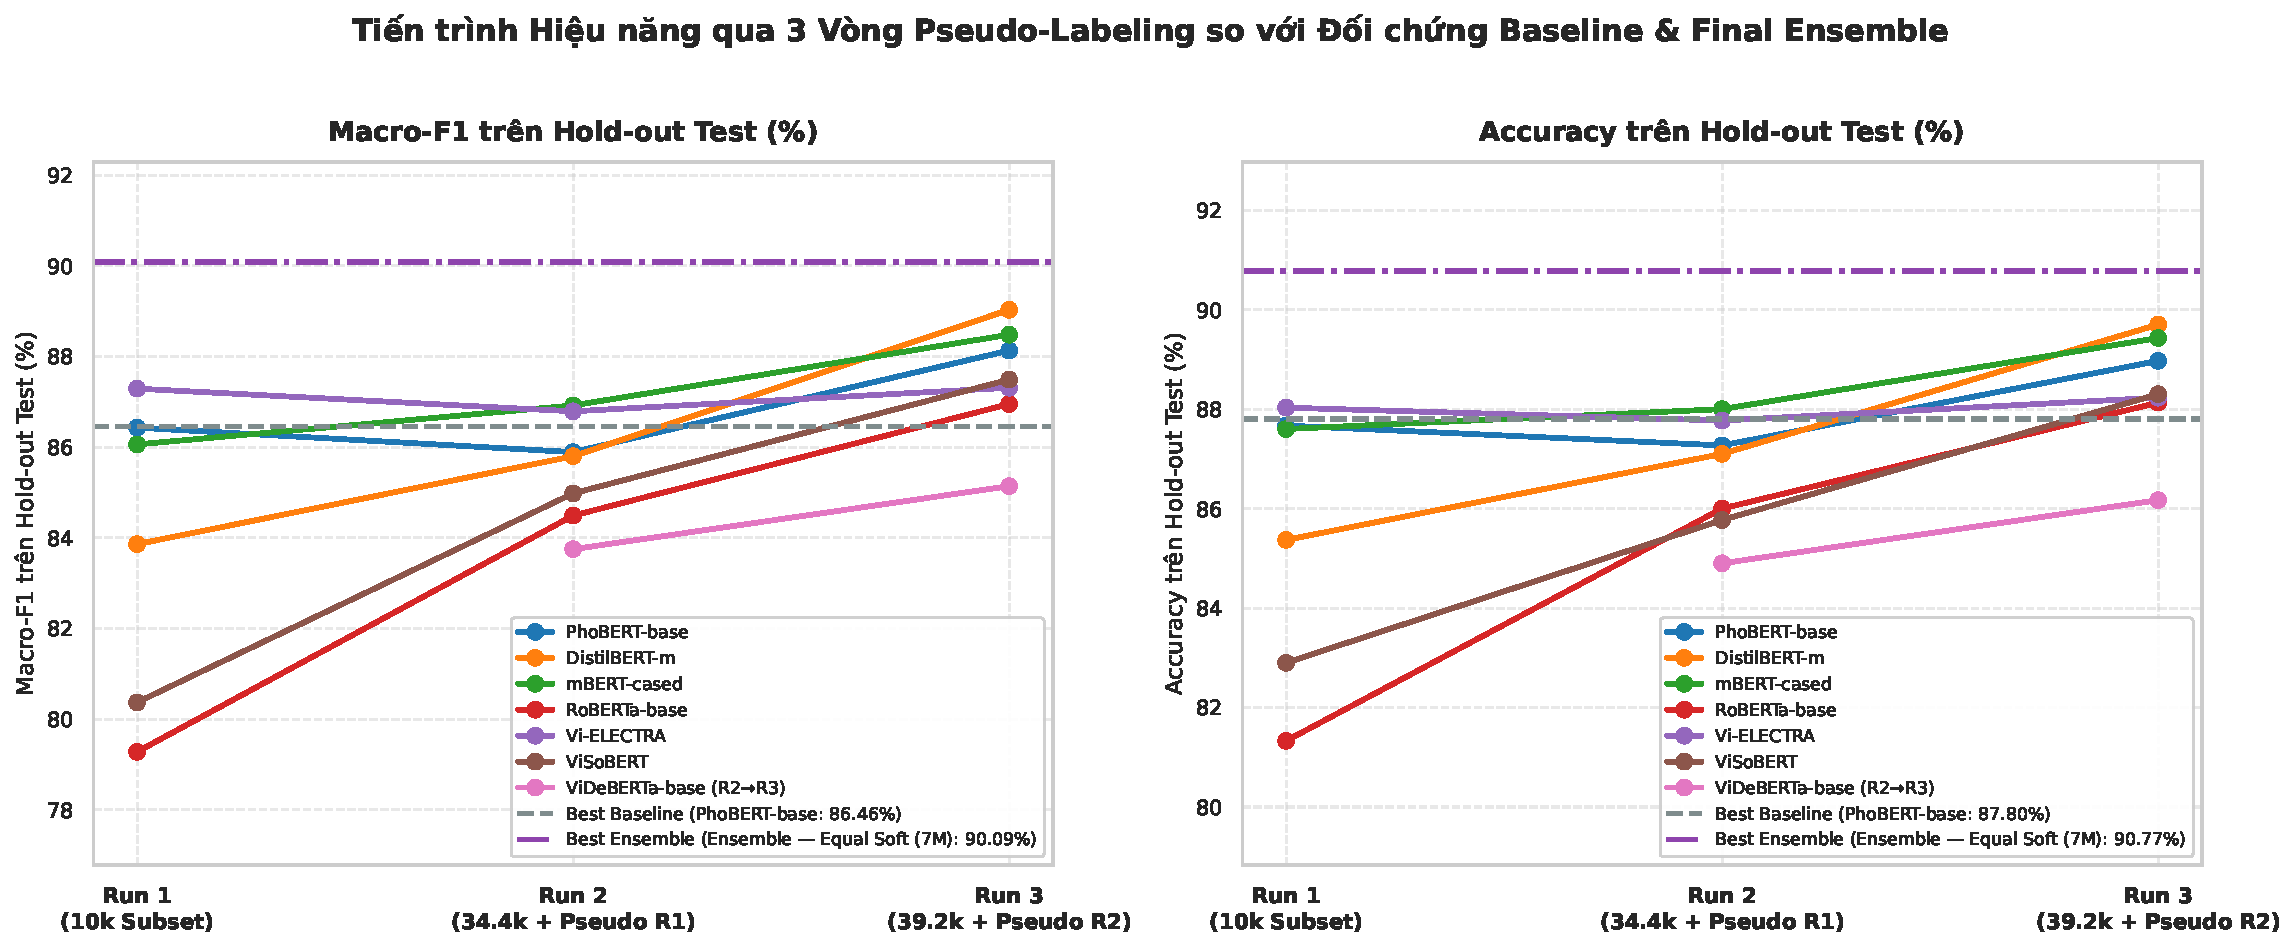
\includegraphics[width=0.96\textwidth]{B8_01_tien_trinh_3_vong_va_ablation.pdf}
  \caption{Tiến trình Macro-F1 và Accuracy qua ba vòng huấn luyện so với mốc đối chứng Baseline và mô hình kết hợp Ensemble cuối cùng.}
  \label{fig:progress}
\end{figure*}

\begin{figure*}[!t]
  \centering
  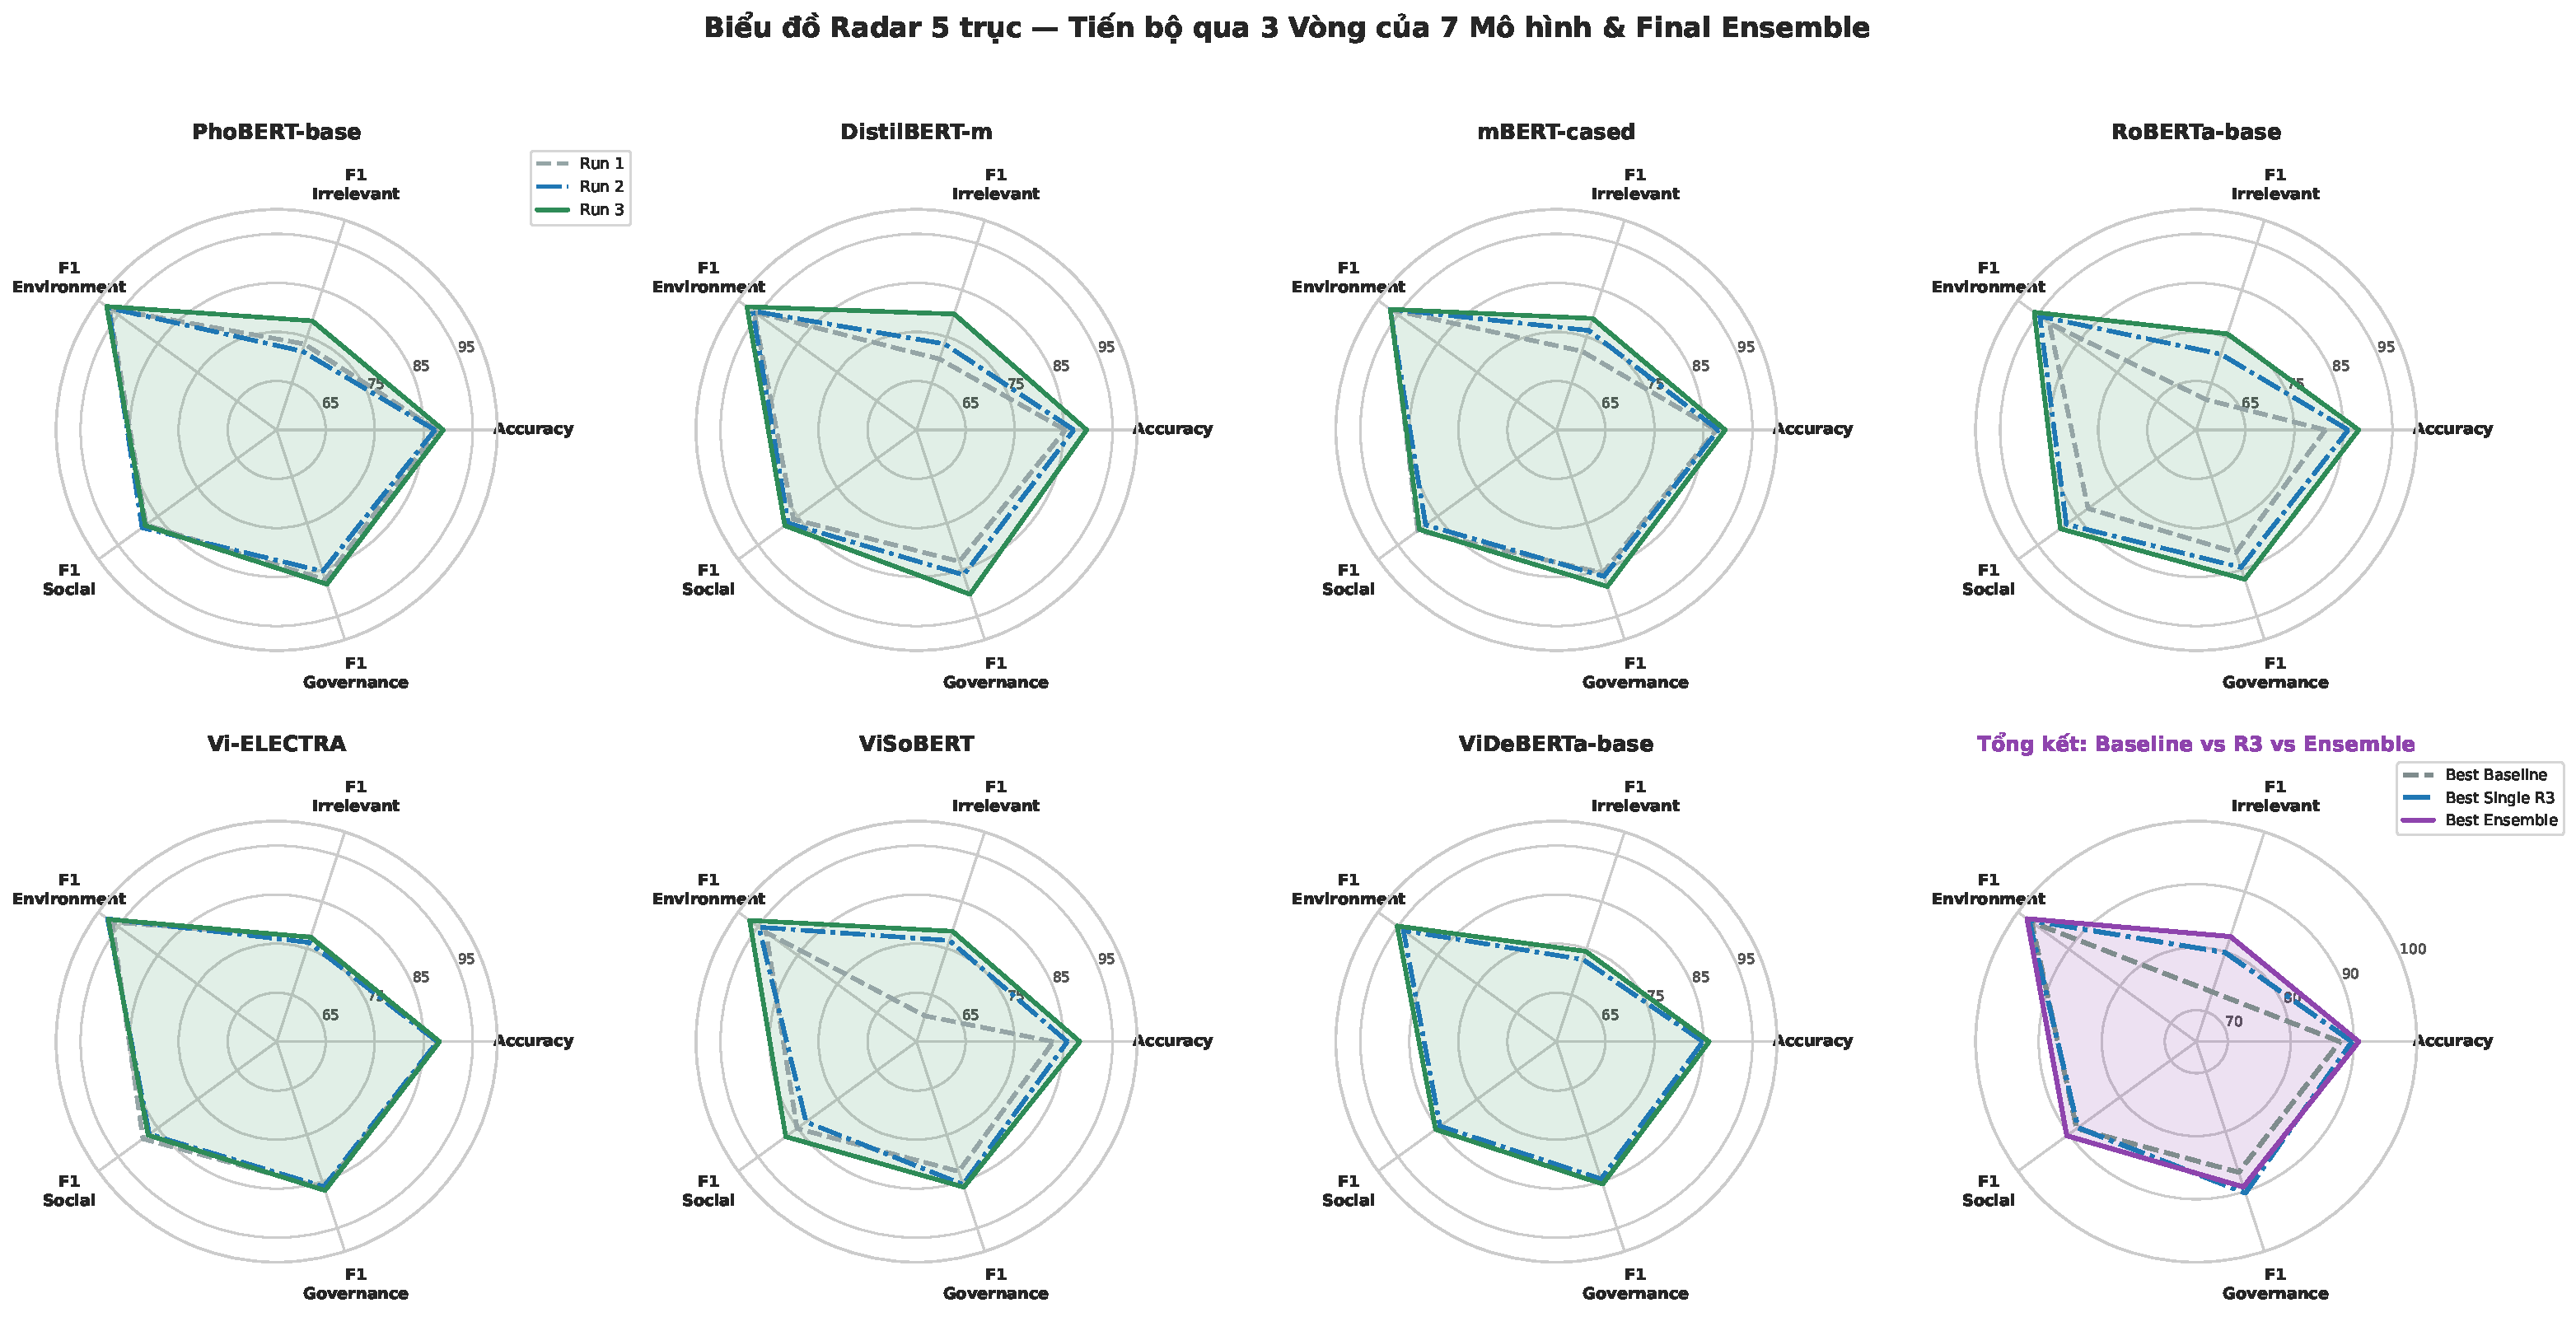
\includegraphics[width=\textwidth]{B8_02_radar_charts_7_models.pdf}
  \caption{Biểu đồ Radar năm trục theo dõi sự thay đổi hiệu năng qua ba vòng của bảy mô hình và so sánh tổng kết giữa Baseline, vòng~3 và Ensemble (ô cuối).}
  \label{fig:radar}
\end{figure*}

% ============================================================================
\section{Thảo luận, hiệu chuẩn xác suất, đánh đổi triển khai và phân tích lỗi}
\label{sec:discussion}

\subsection{Hiệu năng theo từng lớp ESG và cơ chế bổ trợ trên ma trận nhầm lẫn}

Quan sát ô thứ tám trong Hình~\ref{fig:radar}, bản đồ nhiệt theo lớp (Hình~\ref{fig:heatmap}) và ma trận nhầm lẫn song song (Hình~\ref{fig:cm}), sự cải thiện của \code{Equal Soft (7M)} so với mô hình đơn lẻ tốt nhất (\code{DistilBERT-m}) thể hiện rõ ở ba điểm:
\begin{itemize}[leftmargin=*, itemsep=2pt, topsep=2pt]
  \item Giảm hơn một nửa số mẫu \textit{Social} bị dự đoán nhầm sang \textit{Irrelevant} ($91 \rightarrow 39$, tăng Recall lớp \textit{Social} từ $83{,}2\%$ lên $87{,}4\%$ và F1 lên $90{,}39\%$) và giảm số mẫu \textit{Governance} nhầm sang \textit{Irrelevant} ($32 \rightarrow 13$, tăng Recall lớp \textit{Governance} lên $97{,}1\%$).
  \item Cải thiện Precision của lớp \textit{Irrelevant} từ $79{,}4\%$ lên $89{,}2\%$, đưa F1 lớp này từ $73{,}29\%$ (Baseline) và $79{,}87\%$ (\code{DistilBERT-m}) lên $82{,}54\%$ (tăng $+9{,}25$ điểm phần trăm so với mốc Baseline).
  \item Lớp \textit{Environment} đạt mức phân loại chính xác cao nhất với $810/820$ mẫu đúng (Recall $98{,}78\%$, Precision $97{,}59\%$, F1 $98{,}18\%$), phù hợp với hai giả thuyết nêu ra từ phần phân tích khám phá dữ liệu.
\end{itemize}

\begin{figure*}[!t]
  \centering
  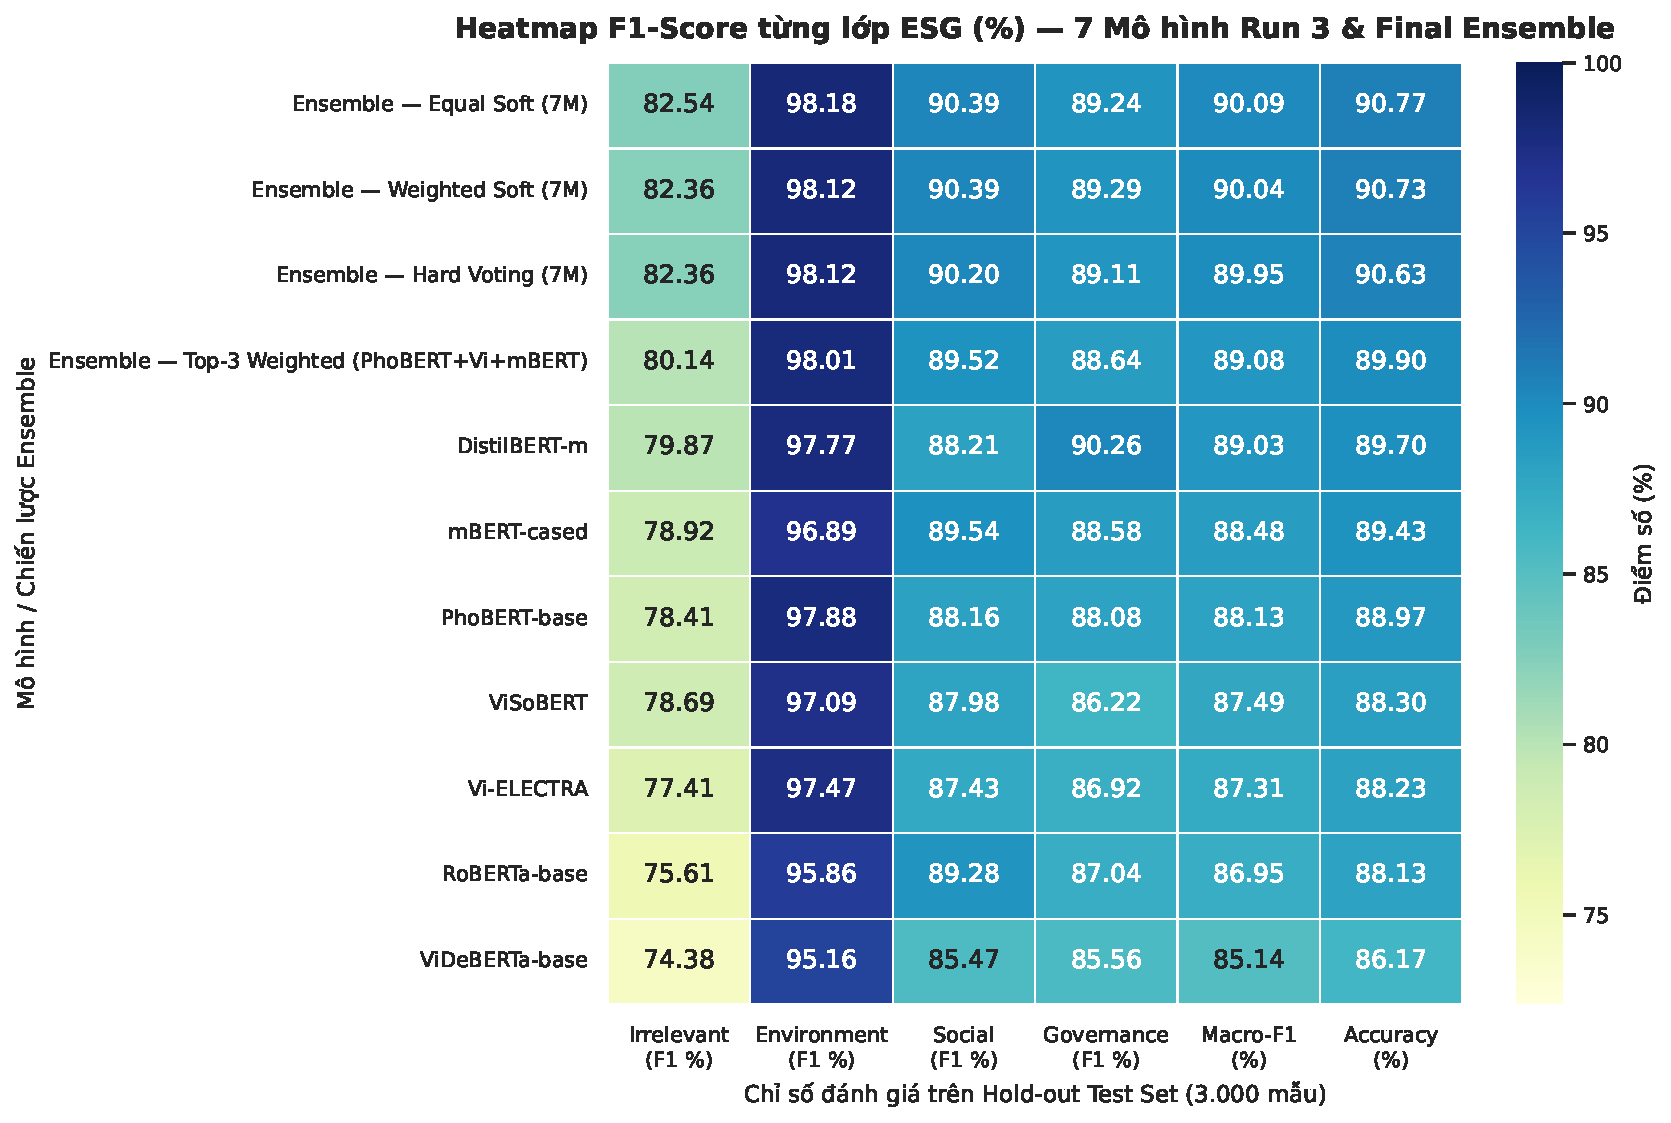
\includegraphics[width=0.88\textwidth]{B8_03_heatmap_f1_theo_lop.pdf}
  \caption{Bản đồ nhiệt F1-Score theo từng lớp ESG (\%) của bảy mô hình vòng~3 và bốn chiến lược Ensemble trên tập kiểm thử.}
  \label{fig:heatmap}
\end{figure*}

\begin{figure*}[!t]
  \centering
  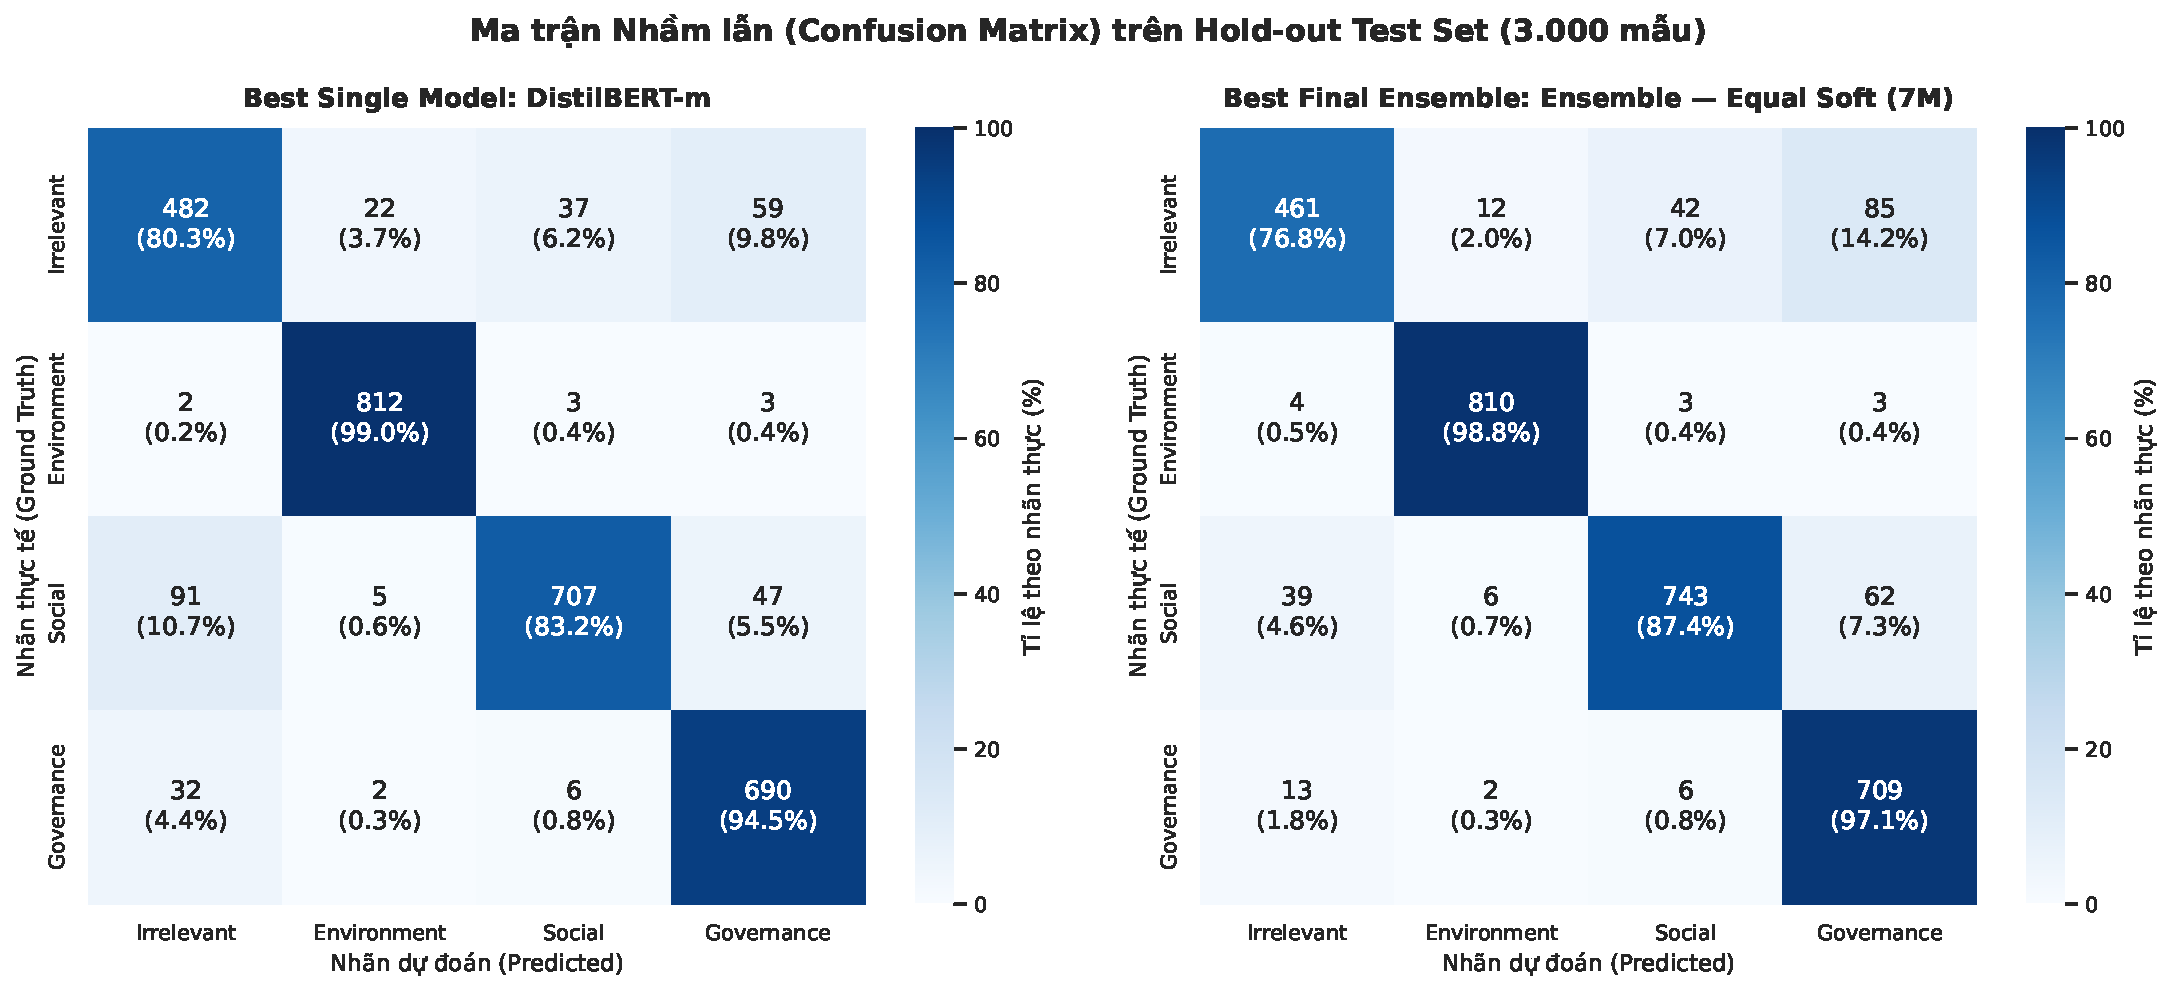
\includegraphics[width=0.96\textwidth]{B8_04_confusion_matrix_best_va_ensemble.pdf}
  \caption{So sánh ma trận nhầm lẫn (số lượng mẫu và Recall theo hàng) giữa mô hình đơn lẻ tốt nhất (\code{DistilBERT-m}) và mô hình Ensemble tốt nhất (\code{Equal Soft 7M}).}
  \label{fig:cm}
\end{figure*}

\subsection{Hiệu chuẩn xác suất và đường biên tối ưu Pareto}

\begin{figure*}[!t]
  \centering
  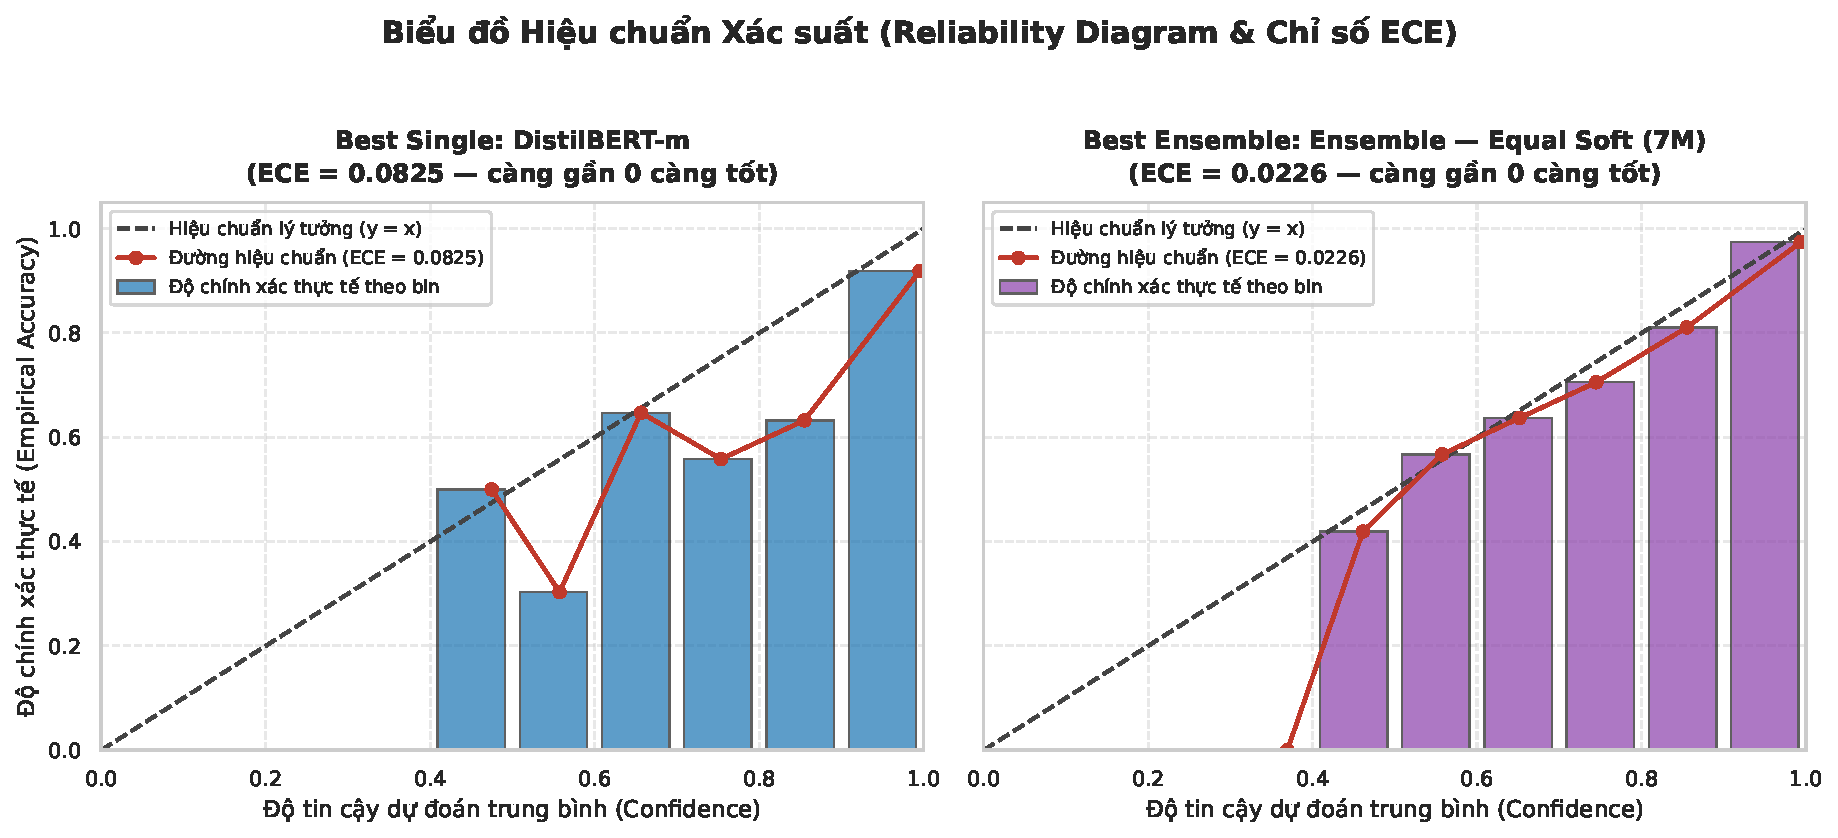
\includegraphics[width=0.94\textwidth]{B8_06_calibration_reliability.pdf}
  \caption{Biểu đồ hiệu chuẩn xác suất (Reliability Diagram): \code{Equal Soft (7M)} bám sát đường chéo lý tưởng $y=x$ và giảm chỉ số ECE từ 0,0825 xuống 0,0226.}
  \label{fig:calibration}
\end{figure*}

\begin{figure*}[!t]
  \centering
  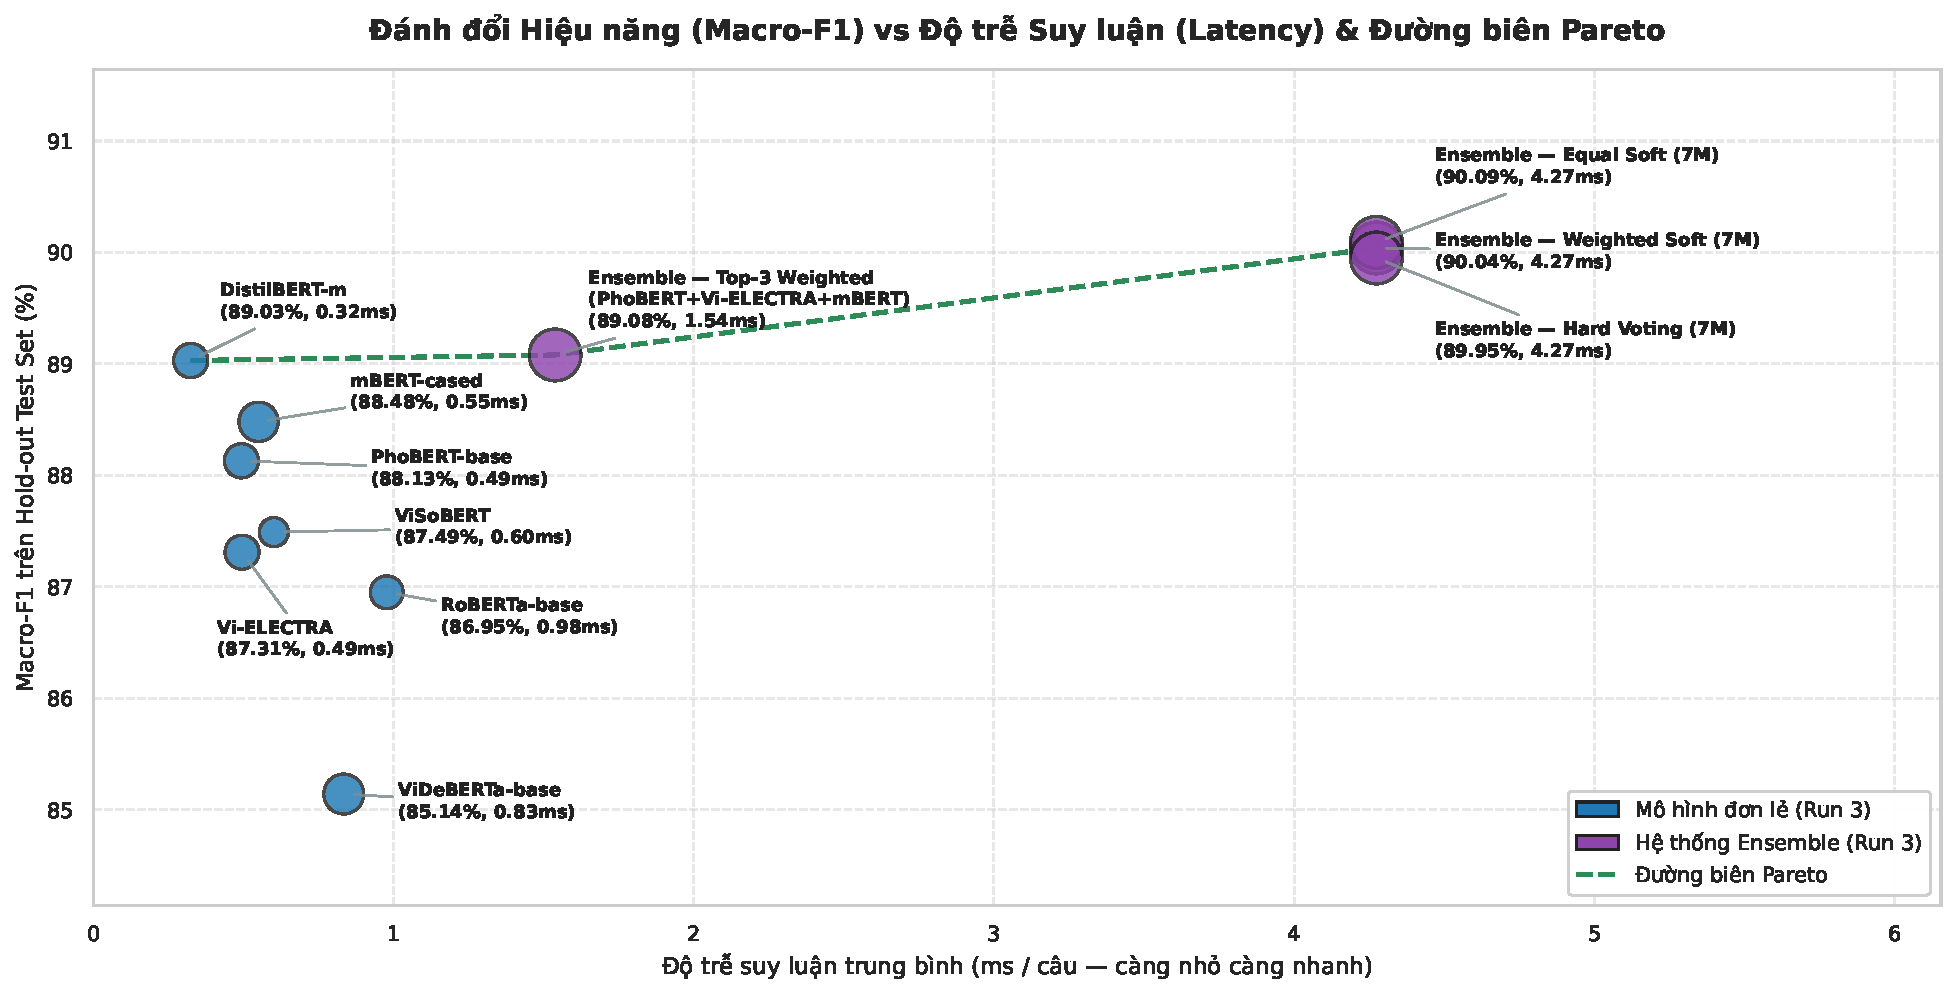
\includegraphics[width=0.96\textwidth]{B8_05_tradeoff_hieu_nang_va_toc_do.pdf}
  \caption{Đánh đổi giữa Macro-F1 và độ trễ suy luận trung bình (ms/câu) trên RTX 5070 cùng đường biên tối ưu Pareto.}
  \label{fig:pareto}
\end{figure*}

\textbf{Hiệu chuẩn xác suất (Hình~\ref{fig:calibration}):} Các mô hình đơn lẻ đều có mức sai số hiệu chuẩn tương đối cao ($\text{ECE} \in [0{,}0825; 0{,}1117]$); ví dụ ở \code{DistilBERT-m}, các dự đoán thuộc khoảng tin cậy $[0{,}5; 0{,}6]$ chỉ đạt độ chính xác thực tế 30\%. Khi lấy trung bình xác suất từ bảy kiến trúc khác nhau, đường hiệu chuẩn của \code{Equal Soft (7M)} bám sát đường chéo $y = x$, giảm ECE xuống 0,0226 (thấp hơn $3{,}6\text{--}4{,}9$ lần so với từng mô hình đơn lẻ). Tại khoảng tin cậy $[0{,}9; 1{,}0]$, 2.316/3.000 mẫu (77,2\% tập kiểm thử) đạt độ chính xác thực tế 97,41\% so với độ tin cậy trung bình 99,35\% (chênh lệch 1,94\%). Đặc tính này thuận lợi cho quy trình kiểm duyệt bán tự động (\textit{Human-in-the-Loop}), trong đó các câu có độ tin cậy $\ge 0{,}90$ được xử lý tự động và chỉ khoảng 22,8\% câu còn lại cần chuyên gia rà soát.

\textbf{Gợi ý cấu hình triển khai theo đường biên Pareto (Hình~\ref{fig:pareto}):}
\begin{enumerate}[leftmargin=*, itemsep=2pt, topsep=2pt]
  \item \textbf{Yêu cầu tốc độ cao hoặc tài nguyên hạn chế:} \code{DistilBERT-m (vòng~3)} đạt 89,03\% Macro-F1 ở độ trễ 0,324~ms/câu (3.085~mẫu/giây, 2,96~GB VRAM), giữ lại 98,8\% mức Macro-F1 của Ensemble 7 mô hình với độ trễ giảm 13,2 lần.
  \item \textbf{Cấu hình cân bằng:} \code{Top-3 Weighted Ensemble} đạt 89,08\% Macro-F1 ở độ trễ 1,54~ms/câu (650~mẫu/giây, $\text{ECE}=0{,}0589$).
  \item \textbf{Yêu cầu độ chính xác và độ hiệu chuẩn cao nhất:} \code{Equal Soft (7M)} đạt 90,09\% Macro-F1, 90,77\% Accuracy và $\text{ECE}=0{,}0226$ với thông lượng 234~mẫu/giây (tương đương khoảng 43 giây cho 10.000 câu trên một GPU RTX 5070).
\end{enumerate}

\subsection{Phân tích lỗi định lượng và định tính}

Trong tổng số 277 mẫu dự đoán sai (9,23\%) của \code{Equal Soft (7M)}, bốn cặp lớp nhầm lẫn đứng đầu chiếm 82,31\% tổng lỗi (Bảng~\ref{tab:errors}). Khảo sát định tính 15 mẫu sai có độ tin cậy cao nhất ($99{,}70\%\text{--}99{,}97\%$) cho thấy ba nguyên nhân chính:

\begin{table}[!t]
\centering
\caption{Phân bố các cặp nhầm lẫn trong 277 mẫu dự đoán sai của \code{Equal Soft (7M)}.}
\label{tab:errors}
\footnotesize
\renewcommand{\arraystretch}{1.15}
\setlength{\tabcolsep}{6pt}
\begin{adjustbox}{max width=\columnwidth}
\begin{tabular}{@{}lcc@{}}
\toprule
\textbf{Cặp nhầm lẫn (Thực $\rightarrow$ Đoán)} & \textbf{Số lỗi} & \textbf{Tỷ trọng} \\
\midrule
Irrelevant $\rightarrow$ Governance & \best{85} & \best{30,69\%} \\
Social $\rightarrow$ Governance & \best{62} & \best{22,38\%} \\
Irrelevant $\rightarrow$ Social & 42 & 15,16\% \\
Social $\rightarrow$ Irrelevant & 39 & 14,08\% \\
Tám cặp còn lại (Environment chỉ có 10 lỗi) & 49 & 17,69\% \\
\midrule
\textbf{Tổng số lỗi trên 3.000 mẫu} & \textbf{277} & \textbf{100,00\%} \\
\bottomrule
\end{tabular}
\end{adjustbox}
\end{table}

\begin{enumerate}[leftmargin=*, itemsep=2pt, topsep=2pt]
  \item \textbf{Dấu hiệu nhiễu nhãn trong tập kiểm thử gốc:} Một số câu có độ tin cậy dự đoán trên 99,8\% mang nội dung phù hợp với nhãn dự đoán của Ensemble hơn nhãn gốc. Ví dụ, dòng \code{2474} (\textit{``trưng bày công nghệ xanh, năng lượng tái tạo và các giải pháp môi trường''}) và dòng \code{413} (\textit{``94\% vật liệu trong bao bì được làm từ vật liệu tái sử dụng, tái chế, có thể phân hủy''}) được gán nhãn gốc \code{Irrelevant} nhưng Ensemble dự đoán \code{Environment} (99,97\% và 99,87\%). Tương tự, dòng \code{185} (\textit{``chiến lược công ty, quản lý rủi ro và quản trị công ty''}) và dòng \code{1022} (\textit{``hệ thống kiểm soát nội bộ hiệu quả''}) được gán gốc \code{Irrelevant} trong khi Ensemble dự đoán \code{Governance} (99,83\%--99,93\%). Điều này gợi ý rằng một phần sai số đo được có thể xuất phát từ nhiễu nhãn trong tập dữ liệu gốc thay vì hạn chế của mô hình.
  \item \textbf{Giao thoa đa nhãn trên biên \textit{Social--Governance} (22,38\% lỗi):} Chẳng hạn, dòng \code{1173} (\textit{``hội đồng quản trị gồm năm phụ nữ, hai người Mỹ gốc Phi...''}) vừa đề cập cơ cấu hội đồng quản trị (\code{Governance}) vừa liên quan đến tính đa dạng nhân sự (\code{Social}); dòng \code{2194} và \code{2874} mô tả cuộc họp hội đồng quản trị xem xét báo cáo văn hóa lao động và an toàn sức khỏe SHEQ/COVID-19. Khi bài toán được xây dựng theo dạng đơn nhãn, mô hình buộc phải chọn một trong hai trụ cột, tạo ra mức sai số nền khó tránh khỏi.
  \item \textbf{Trùng lặp từ vựng tài chính--kế toán (\textit{Irrelevant $\rightarrow$ Governance}, 30,69\% lỗi):} Các câu như dòng \code{1546}, \code{1277} và \code{2694} mô tả chuẩn mực hạch toán, báo cáo tài chính hợp nhất và khoản vay liên công ty có nhiều cụm từ hành chính--pháp lý gần với \code{Governance}, dẫn đến Precision của lớp \code{Governance} thấp hơn hai trụ cột còn lại (82,54\% so với Recall 97,12\%).
\end{enumerate}

% ============================================================================
\section{Kết luận, hạn chế và hướng phát triển}
\label{sec:conclusion}

Nghiên cứu đã xây dựng và đánh giá quy trình phân loại văn bản ESG tiếng Việt bằng phương pháp học bán giám sát lặp kết hợp đồng thuận trên bảy kiến trúc Transformer trong điều kiện kiểm soát không rò rỉ dữ liệu. Qua hai vòng bỏ phiếu đồng thuận và chọn lọc cân bằng lớp, hệ thống đã khai thác 60,4\% kho dữ liệu không nhãn, điều chỉnh tỷ số mất cân bằng $IR$ từ $2{,}29$ về $1{,}35$ và giúp cả ba kiến trúc có đối chứng vượt mốc huấn luyện có giám sát trên 100\% dữ liệu gốc. Hệ thống \code{Equal Soft Ensemble (7M)} đạt 90,77\% Accuracy, 90,09\% Macro-F1 (có ý nghĩa thống kê với $p = 0{,}0161$ so với mô hình đơn lẻ tốt nhất và $p < 10^{-6}$ so với mốc Baseline cao nhất) và chỉ số hiệu chuẩn $\text{ECE} = 0{,}0226$.

\textbf{Hạn chế:} (i) mô hình hóa theo dạng đơn nhãn chưa phản ánh đầy đủ các câu đồng thời thuộc hai trụ cột \textit{Social} và \textit{Governance}; (ii) tập dữ liệu gốc còn tồn tại nhiễu nhãn và một số câu dịch máy chưa tự nhiên; (iii) mô hình kết hợp bảy kiến trúc yêu cầu 988,4 triệu tham số khi triển khai đầy đủ; và (iv) phân loại độc lập từng câu chưa khai thác được ngữ cảnh của đoạn văn chứa câu đó.

\textbf{Hướng phát triển:} (1) Áp dụng kỹ thuật chưng cất tri thức (\textit{Knowledge Distillation})~\cite{hinton2015distilling} từ \code{Equal Soft (7M)} ($\text{ECE}=0{,}0226$) sang một mô hình gọn nhẹ như \code{DistilBERT-m} nhằm dung hòa độ chính xác cao với độ trễ thấp (xấp xỉ 0,32~ms/câu); (2) mở rộng sang bài toán phân loại đa nhãn theo hệ thống tiêu chuẩn GRI/SASB; (3) rà soát nhiễu nhãn bằng phương pháp học tự tin (\textit{Confident Learning})~\cite{northcutt2021confident} kết hợp tối ưu ngưỡng quyết định cho cặp lớp \textit{Irrelevant--Governance}; và (4) tích hợp ngữ cảnh ở cấp độ đoạn văn hoặc tài liệu bằng các mô hình ngôn ngữ có cửa sổ ngữ cảnh dài.

% ============================================================================
\balance
\begin{thebibliography}{16}

\bibitem{huang2023finbert}
A.~H. Huang, H.~Wang, and Y.~Yang, ``FinBERT: A large language model for extracting information from financial text,'' \textit{Contemporary Accounting Research}, vol.~40, no.~2, pp.~806--841, 2023.

\bibitem{guo2017calibration}
C.~Guo, G.~Pleiss, Y.~Sun, and K.~Q. Weinberger, ``On calibration of modern neural networks,'' in \textit{Proc. 34th Int. Conf. Mach. Learn. (ICML)}, PMLR, vol.~70, 2017, pp.~1321--1330.

\bibitem{devlin2019bert}
J.~Devlin, M.-W. Chang, K.~Lee, and K.~Toutanova, ``BERT: Pre-training of deep bidirectional transformers for language understanding,'' in \textit{Proc. NAACL-HLT}, 2019, pp.~4171--4186.

\bibitem{sanh2019distilbert}
V.~Sanh, L.~Debut, J.~Chaumond, and T.~Wolf, ``DistilBERT, a distilled version of BERT: smaller, faster, cheaper and lighter,'' \textit{NeurIPS EMC\textsuperscript{2} Workshop}, arXiv:1910.01108, 2019.

\bibitem{liu2019roberta}
Y.~Liu \textit{et al.}, ``RoBERTa: A robustly optimized BERT pretraining approach,'' \textit{arXiv preprint arXiv:1907.11692}, 2019.

\bibitem{nguyen2020phobert}
D.~Q. Nguyen and A.~T. Nguyen, ``PhoBERT: Pre-trained language models for Vietnamese,'' in \textit{Findings of EMNLP}, 2020, pp.~1037--1042.

\bibitem{clark2020electra}
K.~Clark, M.-T. Luong, Q.~V. Le, and C.~D. Manning, ``ELECTRA: Pre-training text encoders as discriminators rather than generators,'' in \textit{Proc. ICLR}, 2020.

\bibitem{nguyen2023visobert}
N.~Nguyen, T.~Phan, D.-V. Nguyen, and K.~V. Nguyen, ``ViSoBERT: A pre-trained language model for Vietnamese social media text processing,'' in \textit{Proc. EMNLP}, 2023, pp.~5191--5207.

\bibitem{tran2023videberta}
C.~D. Tran, N.~H. Pham, A.~T. Nguyen, T.~S. Hy, and T.~Vu, ``ViDeBERTa: A powerful pre-trained language model for Vietnamese,'' in \textit{Findings of EACL}, 2023, pp.~1071--1078.

\bibitem{dietterich2000ensemble}
T.~G. Dietterich, ``Ensemble methods in machine learning,'' in \textit{Proc. Int. Workshop Multiple Classifier Systems (MCS)}, LNCS, vol.~1857, Springer, 2000, pp.~1--15.

\bibitem{lee2013pseudo}
D.-H. Lee, ``Pseudo-label: The simple and efficient semi-supervised learning method for deep neural networks,'' in \textit{ICML Workshop on Challenges in Representation Learning (WREPL)}, 2013.

\bibitem{grandvalet2004semi}
Y.~Grandvalet and Y.~Bengio, ``Semi-supervised learning by entropy minimization,'' in \textit{Advances in Neural Information Processing Systems (NeurIPS)}, vol.~17, 2004, pp.~529--536.

\bibitem{mcnemar1947note}
Q.~McNemar, ``Note on the sampling error of the difference between correlated proportions or percentages,'' \textit{Psychometrika}, vol.~12, no.~2, pp.~153--157, 1947.

\bibitem{landis1977measurement}
J.~R. Landis and G.~G. Koch, ``The measurement of observer agreement for categorical data,'' \textit{Biometrics}, vol.~33, no.~1, pp.~159--174, 1977.

\bibitem{hinton2015distilling}
G.~Hinton, O.~Vinyals, and J.~Dean, ``Distilling the knowledge in a neural network,'' \textit{arXiv preprint arXiv:1503.02531}, 2015.

\bibitem{northcutt2021confident}
C.~Northcutt, L.~Jiang, and I.~Chuang, ``Confident learning: Estimating uncertainty in dataset labels,'' \textit{Journal of Artificial Intelligence Research (JAIR)}, vol.~70, pp.~1373--1411, 2021.

\end{thebibliography}

\end{document}
